% Options for packages loaded elsewhere
\PassOptionsToPackage{unicode}{hyperref}
\PassOptionsToPackage{hyphens}{url}
\PassOptionsToPackage{dvipsnames,svgnames,x11names}{xcolor}
\PassOptionsToPackage{space}{xeCJK}
\documentclass[
  11pt,
  a4paper,
  oneside,
  openany]{report}
\usepackage{xcolor}
\usepackage[top=25mm,bottom=22mm,left=22mm,right=22mm,headheight=15pt,headsep=7mm]{geometry}
\usepackage{amsmath,amssymb}
\setcounter{secnumdepth}{5}
\usepackage{iftex}
\ifPDFTeX
  \usepackage[T1]{fontenc}
  \usepackage[utf8]{inputenc}
  \usepackage{textcomp} % provide euro and other symbols
\else % if luatex or xetex
  \usepackage{unicode-math} % this also loads fontspec
  \defaultfontfeatures{Scale=MatchLowercase}
  \defaultfontfeatures[\rmfamily]{Ligatures=TeX,Scale=1}
\fi
\usepackage{lmodern}
\ifPDFTeX\else
  % xetex/luatex font selection
  \setmainfont[Path=/Users/zhli/.cache/codex-runtimes/codex-primary-runtime/dependencies/native/libreoffice-headless/libreoffice/LibreOfficeDev.app/Contents/Resources/fonts/truetype/,BoldFont=LiberationSerif-Bold.ttf,ItalicFont=LiberationSerif-Italic.ttf,BoldItalicFont=LiberationSerif-BoldItalic.ttf]{LiberationSerif-Regular.ttf}
  \ifXeTeX
    \usepackage{xeCJK}
    \setCJKmainfont[Path=/usr/local/texlive/2026/texmf-dist/fonts/opentype/public/fandol/,Extension=.otf,UprightFont=*-Regular,BoldFont=*-Bold,ItalicFont=FandolKai-Regular]{FandolSong}
    \setCJKsansfont[Path=/usr/local/texlive/2026/texmf-dist/fonts/opentype/public/fandol/,Extension=.otf,UprightFont=*-Regular,BoldFont=*-Bold,ItalicFont=FandolKai-Regular]{FandolHei}
    \setCJKmonofont[Path=/usr/local/texlive/2026/texmf-dist/fonts/opentype/public/fandol/,Extension=.otf,UprightFont=*-Regular,BoldFont=*-Bold,ItalicFont=FandolKai-Regular]{FandolSong}
  \fi
  \ifLuaTeX
    \usepackage[]{luatexja-fontspec}
    \setmainjfont[Path=/usr/local/texlive/2026/texmf-dist/fonts/opentype/public/fandol/,Extension=.otf,UprightFont=*-Regular,BoldFont=*-Bold,ItalicFont=FandolKai-Regular]{FandolSong}
  \fi
\fi
% Use upquote if available, for straight quotes in verbatim environments
\IfFileExists{upquote.sty}{\usepackage{upquote}}{}
\IfFileExists{microtype.sty}{% use microtype if available
  \usepackage[]{microtype}
  \UseMicrotypeSet[protrusion]{basicmath} % disable protrusion for tt fonts
}{}
\usepackage{setspace}
\makeatletter
\@ifundefined{KOMAClassName}{% if non-KOMA class
  \IfFileExists{parskip.sty}{%
    \usepackage{parskip}
  }{% else
    \setlength{\parindent}{0pt}
    \setlength{\parskip}{6pt plus 2pt minus 1pt}}
}{% if KOMA class
  \KOMAoptions{parskip=half}}
\makeatother
\usepackage{longtable,booktabs,array}
\usepackage{calc} % for calculating minipage widths
% Correct order of tables after \paragraph or \subparagraph
\usepackage{etoolbox}
\makeatletter
\patchcmd\longtable{\par}{\if@noskipsec\mbox{}\fi\par}{}{}
\makeatother
% Allow footnotes in longtable head/foot
\IfFileExists{footnotehyper.sty}{\usepackage{footnotehyper}}{\usepackage{footnote}}
\makesavenoteenv{longtable}
\setlength{\emergencystretch}{3em} % prevent overfull lines
\providecommand{\tightlist}{%
  \setlength{\itemsep}{0pt}\setlength{\parskip}{0pt}}
\usepackage{amsmath,amssymb,booktabs,longtable,array,graphicx,caption,fancyhdr,xcolor,float,titlesec,tcolorbox,enumitem,needspace}
\definecolor{NoteBlue}{HTML}{24364B}
\definecolor{NoteTeal}{HTML}{20667C}
\definecolor{NotePale}{HTML}{EFF5F7}
\setlength{\emergencystretch}{3em}
\setlength{\parindent}{2em}
\setlength{\parskip}{0.28em}
\setlist{nosep,leftmargin=2em,topsep=0.3em}
\setcounter{tocdepth}{1}
\renewcommand{\contentsname}{目录}
\renewcommand{\figurename}{图}
\renewcommand{\tablename}{表}
\titleformat{\chapter}[hang]{\sffamily\bfseries\color{NoteBlue}\fontsize{21}{27}\selectfont}{第\ \thechapter\ 章}{0.8em}{}
\titleformat{name=\chapter,numberless}[hang]{\sffamily\bfseries\color{NoteBlue}\fontsize{21}{27}\selectfont}{}{0pt}{}
\titlespacing*{\chapter}{0pt}{4pt}{24pt}
\titleformat{\section}{\sffamily\bfseries\color{NoteBlue}\fontsize{14}{20}\selectfont}{\thesection}{0.7em}{}
\titleformat{\subsection}{\sffamily\bfseries\color{NoteBlue}\fontsize{11.5}{16}\selectfont}{\thesubsection}{0.7em}{}
\titlespacing*{\section}{0pt}{1.1em}{0.45em}
\titlespacing*{\subsection}{0pt}{0.8em}{0.3em}
\captionsetup{font=small,labelfont=bf,justification=justified,singlelinecheck=false,skip=6pt}
\setlength{\intextsep}{9pt}
\pagestyle{fancy}
\fancyhf{}
\fancyhead[L]{\small\color{NoteBlue}探测器中的信号形成}
\fancyhead[R]{\small\color{NoteBlue}L3\quad 有电导介质与动态权重场}
\fancyfoot[C]{\small\thepage}
\renewcommand{\headrulewidth}{0.3pt}
\renewcommand{\chaptermark}[1]{\markboth{\thechapter\quad #1}{}}
\fancypagestyle{plain}{\fancyhf{}\fancyfoot[C]{\small\thepage}\renewcommand{\headrulewidth}{0pt}}
\newtcolorbox{notebox}[1]{colback=NotePale,colframe=NoteTeal,colbacktitle=NoteTeal,coltitle=white,title=#1,fonttitle=\sffamily\bfseries,boxrule=0.4pt,arc=1mm,left=8pt,right=8pt,top=5pt,bottom=5pt,before skip=9pt,after skip=9pt}
\newcommand{\sourcepages}[1]{{\small\color{NoteTeal}原稿对应：第 #1 页}\par\vspace{8pt}}
\newcommand{\fig}[4]{\begin{figure}[H]\centering\includegraphics[width=#2\linewidth]{../l3_curated_figures/#1.pdf}\caption{#3}\label{fig:#1}\end{figure}}
\numberwithin{equation}{chapter}
\AtBeginDocument{\renewcommand{\maketitle}{}}
\usepackage{bookmark}
\IfFileExists{xurl.sty}{\usepackage{xurl}}{} % add URL line breaks if available
\urlstyle{same}
\hypersetup{
  pdftitle={探测器中的信号形成（L3）},
  pdfauthor={探测器信号形成课程讲义},
  colorlinks=true,
  linkcolor={NoteTeal},
  filecolor={Maroon},
  citecolor={Blue},
  urlcolor={NoteTeal},
  pdfcreator={LaTeX via pandoc}}

\title{探测器中的信号形成（L3）}
\author{探测器信号形成课程讲义}
\date{}

\begin{document}
\maketitle

\setstretch{1.17}
\begin{titlepage}
\thispagestyle{empty}
\vspace*{20mm}
{\sffamily\color{NoteTeal}\large DETECTOR SIGNAL FORMATION\par}
\vspace{13mm}
{\sffamily\bfseries\color{NoteBlue}\fontsize{29}{38}\selectfont 探测器中的信号形成\par}
\vspace{7mm}
{\sffamily\Large 有电导介质、动态权重场与读出网络\par}
\vspace{10mm}
{\large 第 3 册\quad 中文讲义\par}
\vspace{22mm}
\noindent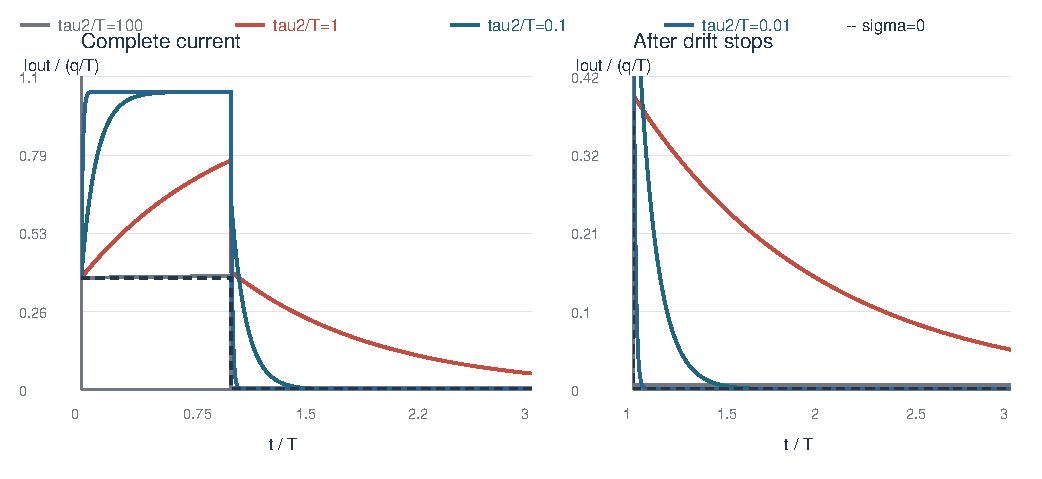
\includegraphics[width=0.94\linewidth]{../l3_curated_figures/planar_pulses.pdf}
\vfill
{\color{NoteBlue}高年级本科与研究生课程\par}
\end{titlepage}
\pagenumbering{roman}

\chapter*{记号与参考方向}\label{ux8bb0ux53f7ux4e0eux53c2ux8003ux65b9ux5411}
\addcontentsline{toc}{chapter}{记号与参考方向}

有限电导允许介质在载流子运动后继续重新分配电荷。因此需要区分真实场、辅助场的时间响应，以及外部网络最后读到的电流或电压。这里采用电准静态、固定工作点附近的线性响应；位移电流保留，而沿长导体的传播延迟不包含在集中节点模型中。

以 \(I_{{\rm out},n}\)
表示从探测器向外部读出网络输出的源电流，\(Q_{g,n}\)
表示接地端供给到电极及相接介质的累计电荷变化，均不含静态偏置背景：

\[
I_{{\rm out},n}=-\frac{dQ_{g,n}}{dt},\qquad
i_{S,n}=\frac{dQ_{g,n}}{dt}=-I_{{\rm out},n}.
\]

在无电导、无色散且电极电势固定的极限，\(i_{S,n}=q\mathbf E_{w,n}\cdot\mathbf v\)，\(\mathbf E_{w,n}=-\nabla\varphi_{w,n}\)。以相反方向定义电源侧电荷时，\(Q_{S,n}=-Q_{g,n}\)。端口累计量
\(Q_g\)
一般不等于金属表面此刻储存的自由电荷，因为电荷还可以继续流入导电介质。

\begin{longtable}[]{@{}
  >{\raggedright\arraybackslash}p{(\linewidth - 2\tabcolsep) * \real{0.5000}}
  >{\raggedright\arraybackslash}p{(\linewidth - 2\tabcolsep) * \real{0.5000}}@{}}
\toprule\noalign{}
\begin{minipage}[b]{\linewidth}\raggedright
记号
\end{minipage} & \begin{minipage}[b]{\linewidth}\raggedright
含义及单位
\end{minipage} \\
\midrule\noalign{}
\endhead
\bottomrule\noalign{}
\endlastfoot
\(q,\rho,\rho_e,\rho_0\) &
带符号点电荷、物理自由电荷密度、外加源密度、工作点空间电荷 \\
\(\rho_R,\sigma,R_\square\) & 体电阻率、电导率、方块电阻；\(\Omega\)
m、S/m、\(\Omega/\square\) \\
\(s,\omega,\nu\) & Laplace 变量、角频率、普通频率；适当收敛条件下
\(s=i\omega\)，\(\omega=2\pi\nu\) \\
\(w_n(\mathbf r,s),\mathbf e_n=-\nabla w_n\) &
电压边界的传递函数及其场；频域单位为 1、m\(^{-1}\) \\
\(\mathbf h_n,\mathbf H_n=V_0\mathbf h_n\) &
归一化阶跃场响应及带测试电压的阶跃场响应 \\
\(\mathbf W_n=V_0\mathbf e_n(\mathbf r,t)\) &
含瞬时项的电流权重向量，单位 V/(m s) \\
\(\mathbf K_n\) & 电流冲激、累计电荷阶跃激励产生的场变化，单位 V/m \\
\(\mathbf c,\mathbf Y,\mathbf z\) & Maxwell
电容矩阵、节点导纳矩阵、节点阻抗矩阵 \\
\(Z_{nm},Z_{n0}\) & 两节点之间及节点至参考地的实际等效支路阻抗 \\
\end{longtable}

阶跃响应、冲激响应和频域传递函数不是同一个量。瞬时空间耦合对应时域冲激核，具有记忆的耦合还含延迟部分；卷积中的空间位置须取载流子在过去时刻的位置。

\clearpage
\tableofcontents
\clearpage
\pagenumbering{arabic}

\chapter{从静态权重场到电准静态问题}\label{chap-eqs}

\section{有限电导与非理想端口}\label{sec-assumptions}

金属电极仍近似为等势面，但电极之间可以存在有限电导，端口也可以连接有限阻抗。因而固定几何的静态权重场不再足以确定整个波形：介质电荷重排和外部电路都可能引入时间响应。

电阻材料可以承担高压分配、放电保护或横向信号展宽等作用。RPC
的玻璃电极、未完全耗尽的硅、附加在读出面上的电阻膜，都有有限电导。粒子产生的载流子运动时，不仅直接改变金属电极上的感应，还驱动介质中的欧姆电流。这个欧姆电流再次改变电荷分布，形成随时间演化的屏蔽。把介质仅替换成一个较大的介电常数，不能描述这种记忆效应。

这里的主线仍是线性响应：先求没有待测电荷时的辅助问题，再把辅助响应与真实载流子轨迹组合。区别在于，辅助问题不再只给一个空间函数，而给一个同时依赖位置和延迟时间的响应核。

\section{介电质中的静电叠加}\label{sec-dielectric}

设 \(A_n\) 为第 \(n\) 个金属电极的表面，\(n=0,\ldots,N\)，其中 0
包含参考外边界。线性、各向同性介质中的势满足

\begin{equation}
\nabla\cdot[\varepsilon(\mathbf r)\nabla\varphi(\mathbf r)]
=-\rho(\mathbf r),\qquad \varphi|_{A_n}=V_n.
\end{equation}

构造两类辅助解。第一类 \(\varphi_0\)
保留体电荷，但把所有电极接地；第二类 \(\psi_n\) 移去体电荷，仅把电极
\(n\) 设为测试电压 \(V_w\)，其余设为零：

\begin{equation}
\begin{aligned}
\nabla\cdot(\varepsilon\nabla\varphi_0)&=-\rho,&\varphi_0|_{A_m}&=0,\\
\nabla\cdot(\varepsilon\nabla\psi_n)&=0,&\psi_n|_{A_m}&=V_w\delta_{mn}.
\end{aligned}
\end{equation}

由线性叠加及边值问题的唯一性，完整解为

\begin{equation}
\varphi(\mathbf r)=\varphi_0(\mathbf r)
+\sum_{n=0}^{N}\frac{V_n}{V_w}\psi_n(\mathbf r).
\end{equation}

\fig{dielectric_basis}{0.98}{介质中任意电位和体电荷的静电问题，可分解为一个接地体电荷问题及四个电极边界基函数。图中 0 为外部边界，前三个为内部电极；各辅助图的体电荷项应为零，只有 $\varphi_0$ 保留源。}{}

由此可见，介电质本身不破坏静态 Shockley--Ramo
定理；它改变的是权重势的空间形状。对每个金属表面取法向 \(\mathbf n_m\)
\textbf{由金属指向介质}，则表面电荷及 Maxwell 电容系数为

\begin{equation}
Q_m=\oint_{A_m}\varepsilon\mathbf E\cdot\mathbf n_m\,dA,
\qquad
c_{mn}=\frac{1}{V_w}\oint_{A_m}\varepsilon\mathbf E_n\cdot\mathbf n_m\,dA,
\quad \mathbf E_n=-\nabla\psi_n.
\end{equation}

这个法向选择使自电容系数为正，互电容系数一般为负。若用``介质区域的外法向''，它在内电极表面与这里法向相反，表面积分前必须补一个负号。不能只抄公式而不声明法向。

\section{体电阻率、方块电阻与电流密度}\label{sec-resistivity}

体电阻率 \(\rho_R\) 的 SI 单位为 \(\Omega\) m，探测器材料文献常用
\(\Omega\) cm。换算关系及均匀样品的电阻为

\begin{equation}
\sigma=\frac{1}{\rho_R},\quad [\sigma]=\mathrm{S/m},\qquad
1\ \Omega\,\mathrm{cm}=10^{-2}\ \Omega\,\mathrm m,\qquad
R_{\rm bulk}=\rho_R\frac{L}{A}.
\end{equation}

对厚度 \(h\) 远小于横向尺寸的均匀薄膜，定义方块电阻

\begin{equation}
R_\square=\frac{\rho_R}{h},\qquad
R_{\rm film}=R_\square\frac{a}{b}.
\end{equation}

电流沿长度 \(a\) 方向流动，横向宽度为
\(b\)。任何同一材料、同一厚度的正方形，端到端电阻均为
\(R_\square\)；``每方块''提醒我们这是几何比例而不是每平方米。对于空间非均匀的材料，必须使用局域关系

\begin{equation}
\mathbf j_{\sigma}(\mathbf r,t)=\sigma(\mathbf r)\mathbf E(\mathbf r,t)
=-\sigma(\mathbf r)\nabla\varphi(\mathbf r,t).
\end{equation}

\fig{resistivity}{0.88}{体电阻与薄膜方块电阻的几何定义。左侧沿 $L$ 流动、截面积为 $A$；右侧沿 $a$ 流动、宽度为 $b$。电导率单位为 S/m，元件电导单位为 S。}{}

\section{从守恒方程得到电准静态方程}\label{sec-eqs-derive}

把由粒子电荷或外部注入规定的电流密度称为外加源电流
\(\mathbf j_e\)，它与介质的欧姆电流不同。总自由电流为

\begin{equation}
\mathbf j=\sigma\mathbf E+\mathbf j_e,\qquad
\nabla\cdot\mathbf j=-\partial_t\rho,\qquad
\nabla\cdot\mathbf j_e=-\partial_t\rho_e.
\end{equation}

\(\rho\) 是通过 Gauss 定律观察到的物理自由电荷密度；\(\rho_e\)
是驱动问题的外加源。对时间不变的 \(\varepsilon,\sigma\)，将 Poisson
方程对时间求导，再代入电荷守恒，得到

\begin{equation}
\begin{aligned}
\nabla\cdot[\varepsilon\nabla\partial_t\varphi]
&=-\partial_t\rho=\nabla\cdot\mathbf j,\\
\nabla\cdot[\varepsilon\nabla\partial_t\varphi
+\sigma\nabla\varphi]&=-\partial_t\rho_e.
\end{aligned}
\end{equation}

\fig{impressed_current}{0.45}{介质中的真实电场驱动欧姆电流，同时还可以存在独立规定的外加源电流 $\mathbf j_e$。两者一起满足物理电荷的连续性方程。}{}

这也可以直接从 Maxwell 方程理解。在线性介质中

\begin{equation}
\begin{aligned}
\nabla\cdot\mathbf D&=\rho,&\nabla\cdot\mathbf B&=0,\\
\nabla\times\mathbf E&=-\partial_t\mathbf B,&
\nabla\times\mathbf H&=\partial_t\mathbf D+\mathbf j_e+\sigma\mathbf E,\\
\mathbf D&=\varepsilon\mathbf E,&\mathbf B&=\mu\mathbf H.
\end{aligned}
\end{equation}

电准静态（electroquasistatic，EQS）近似认为，在所研究的空间尺度和时间尺度上，磁感应对电场的反馈可以忽略，因而
\(\nabla\times\mathbf E\simeq0\)，可以使用标量势。它并没有删除位移电流。对
Ampère--Maxwell 方程取散度，利用旋度的散度为零，仍得到上述守恒方程。

\begin{notebox}{近似的边界}
“准静态”不等于“所有量不随时间变化”。这里可描述很强的电荷松弛和快速脉冲，但假定传播延迟与电感反馈相对于所关心的响应可忽略。若结构长度对应的传播时间不可忽略，或读出导体须作为传输线处理，不能仅用这里的瞬时空间边值问题解决。
\end{notebox}

\section{Laplace 变换：把时间微分变为代数}\label{sec-laplace}

对双边 Laplace 变换，若令所有新增扰动在 \(t<0\) 为零；这样双边变换与从
\(0^-\) 开始的单边变换一致，并且能正确包含 \(t=0\) 的冲激。定义

\begin{equation}
F(s)=\int_{-\infty}^{\infty}f(t)e^{-st}dt,
\qquad
f(t)=\frac{1}{2\pi i}\int_{c-i\infty}^{c+i\infty}F(s)e^{st}ds.
\end{equation}

竖直积分线的实部 \(c\)
位于收敛域中。若虚轴属于适当的收敛边界，\(F(i\omega)\) 就是 Fourier
变换：

\begin{equation}
F(i\omega)=\int_{-\infty}^{\infty}f(t)e^{-i\omega t}dt,
\qquad
f(t)=\frac{1}{2\pi}\int_{-\infty}^{\infty}F(i\omega)e^{i\omega t}d\omega.
\end{equation}

常用变换性质如下。表中 \(a>0\)，\(n\)
为非负整数，\((f*g)(t)=\int f(t-u)g(u)du\)。

\begin{longtable}[]{@{}ll@{}}
\toprule\noalign{}
时域运算 & Laplace 域对应 \\
\midrule\noalign{}
\endhead
\bottomrule\noalign{}
\endlastfoot
\(af+bg\) & \(aF+bG\) \\
\(f*g\) & \(FG\) \\
\(d^nf/dt^n\) & \(s^nF\)；按零初值或完整分布导数理解 \\
\(\int_{-\infty}^{t}f(u)du\) & \(F/s\) \\
\(f(t-t_0)\) & \(e^{-st_0}F(s)\) \\
\(f(at)\) & \(F(s/a)/a\) \\
\(e^{-s_0t}f(t)\) & \(F(s+s_0)\) \\
\(t^nf(t)\) & \((-1)^nd^nF/ds^n\) \\
初值 \(f(0^+)\) &
\(\lim_{s\to\infty}sF(s)\)，要求无初始冲激且初值存在 \\
终值 \(f(\infty)\) &
\(\lim_{s\to0}sF(s)\)，要求满足终值定理的稳定性条件 \\
\end{longtable}

例如使用单边变换且初值不为零时，\(\mathcal L\{f'\}=sF-f(0^-)\)，不能漏掉初值项。终值定理也不能应用于持续振荡或发散响应；常见的充分条件是
\(sF(s)\) 的极点均位于左半平面。能量守恒形式的 Parseval 关系为

\begin{equation}
\int_{-\infty}^{\infty}|f(t)|^2dt
=\frac{1}{2\pi}\int_{-\infty}^{\infty}|F(i\omega)|^2d\omega
=\int_{-\infty}^{\infty}|F(i2\pi\nu)|^2d\nu.
\end{equation}

对实信号，频谱模平方关于零频对称，最后一项也可写为正频率积分的两倍。复信号必须保留模平方与双边频谱。

\section{核心替换：从静电解生成时间响应}\label{sec-epsilon-effective}

对电准静态方程进行零初值 Laplace 变换，并除以 \(s\)，得到

\begin{equation}
\nabla\cdot\left[\left(\varepsilon(\mathbf r)+\frac{\sigma(\mathbf r)}s\right)
\nabla\Phi(\mathbf r,s)\right]=-\rho_e(\mathbf r,s).
\end{equation}

它与静电 Poisson
方程的结构相同。因此可以先求绝缘介质的静电边值解，再作替换

\begin{equation}
\varepsilon\longrightarrow\varepsilon_{\rm eff}(s)
=\varepsilon+\frac\sigma s,\qquad
\rho_e(t)\longrightarrow\rho_e(s),\qquad
V_n(t)\longrightarrow V_n(s),
\end{equation}

最后反变换到时域。这个 \(\varepsilon_{\rm eff}\)
是把电导并入边值算符的有效量，不意味着物理自由电荷应由它直接按静电公式解释。两类密度仍分别满足

\begin{equation}
\rho(\mathbf r,s)=-\nabla\cdot(\varepsilon\nabla\Phi),
\qquad
\rho_e(\mathbf r,s)=-\nabla\cdot(\varepsilon_{\rm eff}\nabla\Phi).
\end{equation}

后续例子将反复展示这个差别：外加源给定的电荷可以保持不变，而物理局域净电荷因欧姆输运而衰减。若材料本身具有线性色散，可以把
\(\varepsilon,\sigma\) 进一步写为位置和 \(s\)
的函数；这意味着时域中的本构关系也需要卷积，不再是简单的瞬时乘法。

\chapter{均匀介质与界面上的电荷松弛}\label{chap-relaxation}

\section{点电荷突然注入均匀导电介质}\label{sec-point-relaxation}

先考虑均匀介质中的局域注入：在无限均匀介质的原点，于 \(t=0\) 注入电荷
\(Q\)。把这个驱动写为

\begin{equation}
\rho_e(\mathbf r,t)=Q\delta^{(3)}(\mathbf r)\Theta(t),\qquad
\rho_e(\mathbf r,s)=\frac{Q}{s}\delta^{(3)}(\mathbf r).
\end{equation}

绝缘介质中的静态势为 \(Q/(4\pi\varepsilon r)\)。作有效介电常数替换后，

\begin{equation}
\Phi(r,s)=\frac{Q/s}{4\pi(\varepsilon+\sigma/s)r}
=\frac{Q}{4\pi\varepsilon r}\frac{1}{s+1/\tau},
\qquad \tau=\frac\varepsilon\sigma=\varepsilon\rho_R.
\end{equation}

由 \(\mathcal L^{-1}\{1/(s+a)\}=e^{-at}\Theta(t)\) 得到

\begin{equation}
\varphi(r,t)=\frac{Q}{4\pi\varepsilon r}e^{-t/\tau}\Theta(t),
\qquad
\rho(\mathbf r,t)=Qe^{-t/\tau}\delta^{(3)}(\mathbf r)\Theta(t).
\end{equation}

初始场是未屏蔽的 Coulomb
场；随着导电介质响应，局域净电荷及其电场按同一时间常数衰减。这里
\(\tau\)
是均匀体介质的电荷松弛时间，不是载流子漂移时间，也不是外部放大器的成形时间。

\fig{point_medium}{0.78}{均匀介质中的局域点电荷及径向电流。介质响应由 $\varepsilon$ 与 $\sigma$ 共同决定；相同几何也用于恒定点电流注入的例子。}{}

对任意半径的球面，欧姆电流密度及穿出电流为

\begin{equation}
j_r(r,t)=\sigma E_r=\frac{Q}{4\pi r^2\tau}e^{-t/\tau},
\qquad
I_r(t)=4\pi r^2j_r=\frac Q\tau e^{-t/\tau}.
\end{equation}

因此
\(\int_0^\infty I_r(t)dt=Q\)。指数衰减不表示电荷被毁灭，而是电荷经介质流离考察区域。无限介质加电准静态近似允许任意球面立即出现同一总电流，这是理想边值模型的性质，不是对真实信号无限传播速度的主张。有限系统的电荷最终进入边界或外部电路。

\section{恒定点电流：注入与泄漏达到平衡}\label{sec-dc-injection}

若从 \(t=0\) 起以恒定电流 \(I_0\) 注入，则外加累计电荷为
\(Q_e(t)=I_0t\Theta(t)\)，其变换是 \(I_0/s^2\)。同一静电解给出

\begin{equation}
\Phi(r,s)=\frac{I_0}{4\pi\varepsilon r}\frac{1}{s(s+1/\tau)},
\qquad
\varphi(r,t)=\frac{I_0\tau}{4\pi\varepsilon r}(1-e^{-t/\tau}).
\end{equation}

短时间 \(t\ll\tau\)
时，\(1-e^{-t/\tau}\simeq t/\tau\)，势近似由尚未泄漏的 \(I_0t\)
产生。长时间时

\begin{equation}
\varphi(r,\infty)=\frac{I_0}{4\pi\sigma r},
\qquad 4\pi r^2\sigma E_r(\infty)=I_0.
\end{equation}

势不再无限增长，是因为欧姆流出已经等于注入。把局域有效电荷幅值写为
\(Q_{\rm loc}\)，上述两例恰好对应
\(\dot Q_{\rm loc}+Q_{\rm loc}/\tau=I_{\rm inj}\)
的冲激驱动和阶跃驱动。这只是对该均匀对称解的等效描述，不能据此断言任意分层结构只有一个时间常数。

\fig{relaxation_curves}{0.92}{左：瞬时注入后，局域电荷和径向总电流均指数衰减。右：恒定电流注入时，归一化势从零增长到稳态。横轴均为 $t/\tau$，曲线由正文解析式重绘，不是测量。}{}

\section{两个半空间交界处的点电荷}\label{sec-interface-point}

把空间分成介质 1、2
两个无限半空间，点电荷恰好位于平面界面。绝缘情况下，球对称形式的势仍适用，但一个球面的两个半球分别含有不同介电常数。Gauss
通量给出

\begin{equation}
\varphi(r)=\frac{Q}{2\pi(\varepsilon_1+\varepsilon_2)r}.
\end{equation}

加入 \(\sigma_1,\sigma_2\) 后，对在 \(t=0\) 注入的点电荷，

\begin{equation}
\Phi(r,s)=\frac{Q}{2\pi(\varepsilon_1+\varepsilon_2)r}
\frac1{s+1/\tau_{12}},\qquad
\tau_{12}=\frac{\varepsilon_1+\varepsilon_2}{\sigma_1+\sigma_2}.
\end{equation}

势乘上 \(e^{-t/\tau_{12}}\)。分别积分两个半球上的欧姆电流，

\begin{equation}
I_j(t)=\frac{\sigma_jQ}{\varepsilon_1+\varepsilon_2}e^{-t/\tau_{12}},
\qquad
Q_j=\int_0^\infty I_jdt
=\frac{\sigma_j}{\sigma_1+\sigma_2}Q,\quad j=1,2.
\end{equation}

只要总电导非零，\(Q_1+Q_2=Q\)。介电常数影响初始场和松弛速度，而完整时间积分后的流出份额由两侧电导率之比决定。两边电导均为零时不能套用上述电荷分配的
\(0/0\) 表达；那是电荷不泄漏的静电问题。

\fig{interface_point}{0.77}{界面点电荷的静电场（左）及加入电导后的两个半球电流（右）。对同一半径，场的径向幅值相同，但 $\sigma_1,\sigma_2$ 不同使两侧电流不同。}{}

\section{无限均匀面电荷}\label{sec-interface-sheet}

将点源推广为界面上的均匀面电荷
\(q_s\)。在这里采用的不叠加额外背景场的无限平面解中，上、下两侧场指向相反，幅值相同。边界条件给出

\begin{equation}
|E_1(0^+)|=|E_2(0^+)|=\frac{q_s}{\varepsilon_1+\varepsilon_2},
\qquad
E_{\rm mag}(t)=\frac{q_s}{\varepsilon_1+\varepsilon_2}e^{-t/\tau_{12}}.
\end{equation}

由法向位移通量差得到仍留在界面的净面电荷

\begin{equation}
\bar q_s(t)=(\varepsilon_1+\varepsilon_2)E_{\rm mag}(t)
=q_s e^{-t/\tau_{12}}.
\end{equation}

若下半空间为 \(\varepsilon_1=\varepsilon_0\varepsilon_r\)、电导率
\(\sigma\)，上半空间为真空或近似真空介质且不导电，则
\(\tau_{12}=\varepsilon_0(\varepsilon_r+1)/\sigma\)。这已经不同于孤立均匀体的
\(\varepsilon_0\varepsilon_r/\sigma\)：几何边界及另一侧介质也参与储存电场能。

\fig{interface_sheet}{0.76}{无限界面电荷的两个反向场。右图中两侧的欧姆电流将面电荷带离界面；若上侧绝缘，仅下侧提供泄漏通道。}{}

\section{导电半空间上方的点电荷与逐渐建立的像电荷}\label{sec-image-relaxation}

最后把点电荷移离界面，放在上半空间的 \(z=a>0\)。设柱坐标半径
\(r=\sqrt{x^2+y^2}\)，定义到真实电荷和像位置的距离

\begin{equation}
R_+=\sqrt{r^2+(z-a)^2},\qquad R_-=\sqrt{r^2+(z+a)^2}.
\end{equation}

上半空间为 \(\varepsilon_2\)，下半空间为
\(\varepsilon_1\)。满足界面势连续及法向位移连续的静电解为

\begin{equation}
\begin{aligned}
\varphi_2&=\frac{Q}{4\pi\varepsilon_2}
\left[\frac1{R_+}+\frac{\varepsilon_2-\varepsilon_1}{\varepsilon_1+\varepsilon_2}\frac1{R_-}\right],\quad z>0,\\
\varphi_1&=\frac{Q}{2\pi(\varepsilon_1+\varepsilon_2)}\frac1{R_+},\quad z<0.
\end{aligned}
\end{equation}

两侧势必须满足界面连续性：在 \(z=0\) 有
\(R_+=R_-\)，代入即可验证上下势相等；令 \(\varepsilon_1=\varepsilon_2\)
又恢复无界面点电荷解。

现在令
\(\varepsilon_2=\varepsilon_0\)，\(\varepsilon_1\to\varepsilon_0+\sigma/s\)，且源电荷为
\(Q/s\)。反变换得到

\begin{equation}
\begin{aligned}
\varphi_2(r,z,t)&=\frac{Q}{4\pi\varepsilon_0R_+}
-\frac{Q(1-e^{-t/\tau})}{4\pi\varepsilon_0R_-},\quad z>0,\\
\varphi_1(r,z,t)&=\frac{Qe^{-t/\tau}}{4\pi\varepsilon_0R_+},\quad z<0,
\qquad \tau=\frac{2\varepsilon_0}{\sigma}.
\end{aligned}
\end{equation}

在 \(t=0^+\)，导电介质尚未完成重排，两侧相当于同一种介电质；在
\(t\to\infty\)，下半空间内部场消失，上半空间等效于真实电荷 \(Q\)
与像电荷 \(-Q\)。中间时刻像电荷的等效幅值是
\(-Q(1-e^{-t/\tau})\)。像电荷只是用于表示场的数学构造，不是有一颗粒子在下半空间逐渐``生成''。

\fig{image_geometry}{0.76}{界面外点电荷的静态像电荷构造（左），以及下半空间有电导时的几何（右）。竖轴 $z$ 为界面法向。像位置始终在 $-a$，改变的是其等效幅值。}{}

\chapter{有限层中的空间模与电荷展宽}\label{chap-spreading}

\section{接地平板之间的均匀界面电荷}\label{sec-finite-sheet}

前章中各侧都是无限半空间。真实器件有有限层厚和接地边界，电荷松弛时间因而会依赖几何。取下电极
\(z=-b\)、上电极 \(z=g\)，两电极都接地；界面 \(z=0\) 上放置均匀面电荷
\(q_s\)。下层介电常数 \(\varepsilon_1\)、上层
\(\varepsilon_2\)，\(E_1,E_2\) 都是沿 \(+z\) 的带符号分量。

零总电位差与界面 Gauss 条件分别为

\begin{equation}
bE_1+gE_2=0,\qquad -\varepsilon_1E_1+\varepsilon_2E_2=q_s.
\end{equation}

消去一个场，即得

\begin{equation}
E_1=-\frac{gq_s}{\varepsilon_1g+\varepsilon_2b},\qquad
E_2=\frac{bq_s}{\varepsilon_1g+\varepsilon_2b}.
\end{equation}

因此两个场方向相反，图上的参考箭头不意味着两者数值都为正。令下层为
\(\varepsilon_0\varepsilon_r,\sigma\)，上层为 \(\varepsilon_0,0\)，则

\begin{equation}
E_1(t)=-\frac{gq_s}{\varepsilon_0(\varepsilon_rg+b)}e^{-t/\tau_{\rm u}},\qquad
E_2(t)=\frac{bq_s}{\varepsilon_0(\varepsilon_rg+b)}e^{-t/\tau_{\rm u}},
\quad \tau_{\rm u}=\frac{\varepsilon_0}{\sigma}\left(\varepsilon_r+\frac bg\right).
\end{equation}

当 \(b=g\)
时，时间常数恰好等于前章一个导电、一个绝缘半空间的结果。一般厚度下，不能忽略比值
\(b/g\)。

\fig{finite_layers}{0.92}{两个接地平板之间的界面电荷。左图给出一般两介质几何，右图为这里反复使用的“导电底层加绝缘上层”。箭头表示场分量的参考方向，实际 $E_1<0$、$E_2>0$。}{}

\section{局域点电荷需要一整族松弛时间}\label{sec-finite-point}

在同一几何的界面原点放置点电荷 \(Q\)。此时场不再只沿
\(z\)，横向位置也参与问题。利用轴对称的 Fourier--Bessel
展开，静电势可写为

\begin{equation}
\begin{aligned}
\varphi_1(r,z)&=\frac Q{2\pi}\int_0^\infty J_0(kr)
\frac{4\sinh(kg)\sinh[k(b+z)]}{D_\varepsilon(k)}\,dk,\\
\varphi_2(r,z)&=\frac Q{2\pi}\int_0^\infty J_0(kr)
\frac{4\sinh(kb)\sinh[k(g-z)]}{D_\varepsilon(k)}\,dk,\\
D_\varepsilon(k)&=4\{\varepsilon_1\cosh(kb)\sinh(kg)
+\varepsilon_2\sinh(kb)\cosh(kg)\}.
\end{aligned}
\end{equation}

\(J_0\) 是第一类零阶 Bessel 函数；\(k\)
的量纲为长度的倒数。\(\sinh[k(b+z)]\) 和 \(\sinh[k(g-z)]\)
分别保证两个接地面的势为零；共同分母使界面势连续，并满足点源的位移跳变。

作导电替换，并将有量纲分母 \(D_\varepsilon\) 与无量纲分母分开，定义

\begin{equation}
D_0(k)=\varepsilon_r\cosh(kb)\sinh(kg)+\sinh(kb)\cosh(kg),
\qquad
\tau(k)=\frac{\varepsilon_0}{\sigma}
\left[\varepsilon_r+\frac{\tanh(kb)}{\tanh(kg)}\right].
\end{equation}

对 \(z\) 求负梯度，得到 Laplace 域中的两个法向场：

\begin{equation}
\begin{aligned}
E_{1z}(r,z,s)&=-\frac{Q}{2\pi\varepsilon_0}
\int_0^\infty\frac{kJ_0(kr)\sinh(kg)\cosh[k(b+z)]}{D_0(k)}
\frac{dk}{s+1/\tau(k)},\\
E_{2z}(r,z,s)&=\frac{Q}{2\pi\varepsilon_0}
\int_0^\infty\frac{kJ_0(kr)\sinh(kb)\cosh[k(g-z)]}{D_0(k)}
\frac{dk}{s+1/\tau(k)}.
\end{aligned}
\end{equation}

每一个 \(k\) 都对应一个简单极点，反变换逐模进行：

\begin{equation}
\begin{aligned}
E_{1z}(r,z,t)&=-\frac{Q}{2\pi\varepsilon_0}
\int_0^\infty\frac{kJ_0(kr)\sinh(kg)\cosh[k(b+z)]}{D_0(k)}
e^{-t/\tau(k)}dk,\\
E_{2z}(r,z,t)&=\frac{Q}{2\pi\varepsilon_0}
\int_0^\infty\frac{kJ_0(kr)\sinh(kb)\cosh[k(g-z)]}{D_0(k)}
e^{-t/\tau(k)}dk.
\end{aligned}
\end{equation}

这组式子比``用某一个有效 \(RC\)
替代整块材料''更一般。不同横向波长的电场穿透到边界的程度不同，因此储能和泄漏的比例不同。若
\(b\ne g\)，叠加后的局域场一般不再是单指数。

两个极限尤其重要：

\begin{equation}
\tau(k\to\infty)=\frac{\varepsilon_0}{\sigma}(\varepsilon_r+1),
\qquad
\tau(k\to0)=\frac{\varepsilon_0}{\sigma}\left(\varepsilon_r+\frac bg\right).
\end{equation}

高 \(k\) 对应局部短尺度，远处接地边界的影响减弱，恢复半空间结果；低
\(k\) 对应横向长尺度，恢复均匀面电荷的时间常数。当 \(b=g\)，所有 \(k\)
的时间常数相同。两端数值谁大取决于
\(b/g\)，不能不分几何一概称某一个为``最大时间''。

\fig{mode_times}{0.9}{空间模的松弛时间。示例取 $\varepsilon_r=6$，分别令 $b/g=0.25,1,4$；横轴为 $kg$，纵轴为 $\tau\sigma/\varepsilon_0$。三条曲线的高 $k$ 极限均为 7，低 $k$ 极限分别为 6.25、7、10。}{}

\section{恒定点电流在底电极上的横向分布}\label{sec-dc-spread}

若在界面原点持续注入
\(I_0\)，等待稳态后，电流经电阻体流向底部接地平板。即使注入点很小，收集电流也有有限横向宽度。以流向底板的电流密度幅值
\(i_0(r)\) 表示，可写为

\begin{equation}
i_0(r)=\frac{I_0}{\pi b^2}F(r/b),\qquad
F(x)=\frac12\int_0^\infty\frac{yJ_0(xy)}{\cosh y}\,dy.
\end{equation}

对 \(x>0\)，同一函数也可表示为第二类修正 Bessel 函数 \(K_0\) 的级数：

\begin{equation}
F(x)=\frac\pi2\sum_{n=0}^{\infty}(-1)^n(2n+1)
K_0\!\left(\frac{(2n+1)\pi x}{2}\right),
\qquad
F(x)\underset{x\gg1}{\simeq}\frac{\pi}{2\sqrt{x}}e^{-\pi x/2}.
\end{equation}

后一渐近式来自 \(n=0\) 项及 \(K_0(u)\simeq\sqrt{\pi/(2u)}e^{-u}\)。\(F\)
本身无量纲，故其渐近式中不应再额外出现 \(1/b\)。

图中还比较中心附近的二阶、四阶展开。展开 \(J_0(xy)\) 并逐项积分可得

\begin{equation}
F(x)=\beta(2)-\frac32\beta(4)x^2+\frac{15}{8}\beta(6)x^4+\cdots,
\qquad \beta(p)=\sum_{n=0}^{\infty}\frac{(-1)^n}{(2n+1)^p}.
\end{equation}

这解释了多项式近似只在原点附近有意义；图中二阶曲线变负、四阶曲线向上发散，都是把局部展开外推过远的表现，不是负电流或远处电流增大的物理预测。

\fig{dc_geometry}{0.66}{恒定点电流 $I_0$ 在界面注入，经厚度 $b$ 的导电底层流入接地电极。底面电流密度沿半径扩展。}{}

半径 \(r\) 内的累计电流为

\begin{equation}
\begin{aligned}
I(<r)&=\int_0^r2\pi r'i_0(r')dr'\\
&=I_0\left[1-2\sum_{n=0}^\infty(-1)^n\frac rb
K_1\!\left(\frac{(2n+1)\pi r}{2b}\right)\right].
\end{aligned}
\end{equation}

完整积分应为 \(I_0\)。可写为包含 50\%、90\%、99\% 电流的半径分别约为
\(b,2.3b,3.9b\)。这些是稳态电流的空间包络，并非单颗粒子的随机扩散半径。

\fig{dc_curves}{0.95}{左：底面电流密度的精确解、中心二阶/四阶展开及远场指数近似。右：半径内包含的电流份额。横轴均以层厚 $b$ 归一化；图中保留全部曲线与参考线。}{}

\section{孤立无限电阻膜：展宽不一定是 Gaussian}\label{sec-free-sheet}

现在让电流只在无限薄的电阻膜内横向流动。膜位于 \(z=0\)，方块电阻为
\(R_\square\)，两边都是
\(\varepsilon_0\)，附近没有接地面。于原点瞬时放置 \(Q\)。定义

\begin{equation}
v_R=\frac{1}{2\varepsilon_0R_\square}.
\end{equation}

图中将这个量也写为 \(v\)；这里用 \(v_R\)，避免与粒子漂移速率混淆。对于
\(t>0\)，上下半空间的势为

\begin{equation}
\begin{aligned}
\varphi_-(r,z,t)&=\frac{Q}{4\pi\varepsilon_0\sqrt{r^2+(-z+v_Rt)^2}},\quad z<0,\\
\varphi_+(r,z,t)&=\frac{Q}{4\pi\varepsilon_0\sqrt{r^2+(z+v_Rt)^2}},\quad z>0.
\end{aligned}
\end{equation}

从任一半空间看，势等效于一颗向膜另一侧退离的点电荷。但真实电荷留在膜上横向迁移，\(v_R\)
只是场的等效传播尺度，不是载流子垂直穿膜的速度。

由界面两侧法向位移差，

\begin{equation}
q_s(r,t)=\left.\varepsilon_0\partial_z\varphi_-\right|_{0^-}
-\left.\varepsilon_0\partial_z\varphi_+\right|_{0^+}
=\frac Q{2\pi}\frac{v_Rt}{[r^2+(v_Rt)^2]^{3/2}}.
\end{equation}

\fig{free_sheet}{0.88}{无限电阻膜上的局域电荷，以及观察上半空间时的等效退离点电荷。右图是势的数学表示，不是电荷离开膜的真实轨迹。}{}

直接积分可验证 \(2\pi\int_0^\infty rq_sdr=Q\)，并得到半径内电荷份额

\begin{equation}
\frac{Q(<r,t)}Q=1-\frac{v_Rt}{\sqrt{r^2+(v_Rt)^2}}.
\end{equation}

例如半电荷半径为 \(r_{50}=\sqrt3\,v_Rt\)，随时间线性增长。远处
\(q_s\propto r^{-3}\)，并非 Gaussian
尾；在这个无限理想模型中二阶径向矩发散。因此不能给它强行指定一个
Gaussian 的均方根宽度。

\section{增加接地面后，长时间才出现扩散方程}\label{sec-ground-sheet}

把一个接地平面放在膜下 \(b\) 处，其余条件不变。精确面电荷密度为

\begin{equation}
q_s(r,t)=\frac Q{2\pi b^2}\int_0^\infty\kappa J_0\!\left(\kappa\frac rb\right)
\exp\!\left[-\kappa(1-e^{-2\kappa})\frac t{T_b}\right]d\kappa,
\qquad T_b=\frac b{v_R}=2b\varepsilon_0R_\square.
\end{equation}

\(\kappa=kb\)
是无量纲空间波数。时间增大后，高波数成分先衰减，积分主要来自
\(\kappa\ll1\)。利用 \(1-e^{-2\kappa}\simeq2\kappa\)，指数成为
\(-2\kappa^2t/T_b\)，从而

\begin{equation}
q_s(r,t)\underset{t\gg T_b}{\simeq}
\frac{Q}{8\pi b^2(t/T_b)}
\exp\!\left[-\frac{r^2}{8b^2(t/T_b)}\right]
=\frac{Q}{4\pi D_Rt}\exp\!\left[-\frac{r^2}{4D_Rt}\right],
\quad D_R=\frac{2b^2}{T_b}=\frac b{\varepsilon_0R_\square}.
\end{equation}

\fig{ground_sheet}{0.63}{电阻膜与下方接地面相距 $b$。接地面改变各横向空间模的电场和松弛率，不能只沿用无接地面时的分布。}{}

在横向变化尺度远大于 \(b\) 时，膜与接地面局部近似为单位面积电容
\(C_A=\varepsilon_0/b\)，故 \(q_s\simeq C_AV\)。二维面电流为
\(\mathbf j_s=-(1/R_\square)\nabla_\parallel V\)，连续性方程给出

\begin{equation}
\partial_tq_s=D_R\nabla_\parallel^2q_s,\qquad
D_R=\frac1{R_\square C_A},\qquad \langle r^2\rangle=4D_Rt.
\end{equation}

这不是把电阻性电荷输运直接等同于载流子的热扩散，而是局域电容加横向电阻产生的有效扩散方程。附近接地面使远场相互作用局域化，才让长期分布变成
Gaussian。

\fig{sheet_profiles}{0.88}{两种极限分布的形状比较。左图取 $a=v_Rt$，画出 $2\pi a^2q_s/Q$ 随 $r/a$ 的变化；右图取 $a=\sqrt{4D_Rt}$，画出 $\pi a^2q_s/Q$ 随 $r/a$ 的变化。各自采用自己的特征长度，不能把两幅横轴当成同一物理时间下的相同长度。下方对数纵轴显示幂律尾与 Gaussian 尾的差别。}{}

\chapter{电容、导纳与等效多端口网络}\label{chap-network}

\section{单层平板：表面电荷与端口供给电荷}\label{sec-parallel-rc}

设平板面积 \(A\)、间距 \(d\)，下板电位为零，上板为
\(V(t)\)，板间介质均匀。真实场为 \(E_z=-V/d\)，所以两板瞬时表面电荷为

\begin{equation}
Q_1(t)=-CV(t),\qquad Q_2(t)=CV(t),\qquad C=\frac{\varepsilon A}{d}.
\end{equation}

若介质有电导，还存在从上板流向下板的欧姆电流
\(I_\sigma=\sigma AV/d=V/R\)，其中
\(R=d/(\sigma A)\)。为维持给定电位，外端口流入上板的总电流必须既给表面充电，又补偿泄漏：

\begin{equation}
I_{\rm ext}=\frac{dQ_2}{dt}+I_\sigma=C\frac{dV}{dt}+\frac VR,
\qquad
Y(s)=sC+\frac1R,\qquad Z(s)=\frac1{Y(s)}=\frac R{1+sRC}.
\end{equation}

这就是并联 \(RC\)。与电极之间介质相关的 \(R\) 和 \(C\)
不是任选的拟合参数，而分别由同一几何及 \(\sigma,\varepsilon\) 决定，故
\(RC=\varepsilon/\sigma\)。

\fig{parallel_rc}{0.92}{绝缘平板等效为电容；加入体电导后等效为并联 $RC$。外端口电流 $I$ 与介质欧姆电流 $I_2$ 的差才等于上板表面电荷的变化率。}{}

在零初始扰动下，端口到时刻 \(t\) 的累计供给电荷是

\begin{equation}
Q_{\rm ext}(t)=CV(t)+\int_0^t\frac{V(u)}Rdu.
\end{equation}

它一般不等于
\(Q_2(t)=CV(t)\)。例如保持恒定电压时，表面电荷恒定，而端口累计供给电荷仍因持续泄漏而线性增长。这是开篇对
\(Q_g\) 的定义为何必要的最直接例子。

\section{两层平板：串联层与并联泄漏}\label{sec-two-layer-rc}

取下层厚度 \(b\)、介电常数 \(\varepsilon_1\)，上层厚度 \(g\)、介电常数
\(\varepsilon_2\)；两端电压为 \(V\)。此时界面没有额外源电荷，满足

\begin{equation}
-bE_1-gE_2=V,\qquad -\varepsilon_1E_1+\varepsilon_2E_2=0,
\end{equation}

从而

\begin{equation}
E_1=-\frac{\varepsilon_2V}{\varepsilon_1g+\varepsilon_2b},\qquad
E_2=-\frac{\varepsilon_1V}{\varepsilon_1g+\varepsilon_2b},
\qquad Q_2=-\varepsilon_2E_2A=CV.
\end{equation}

等效电容为两个层电容串联：

\begin{equation}
C_1=\frac{\varepsilon_1A}{b},\quad C_2=\frac{\varepsilon_2A}{g},\qquad
C=\frac{C_1C_2}{C_1+C_2}.
\end{equation}

若下层有 \(\varepsilon_0\varepsilon_r,\sigma\)，上层绝缘且
\(\varepsilon_2=\varepsilon_0\)，则

\begin{equation}
E_2(s)=-\frac{(\varepsilon_0\varepsilon_rs+\sigma)V(s)}
{\varepsilon_0s(b+\varepsilon_rg)+g\sigma},
\qquad I_{\rm ext}(s)=sQ_2(s)=-s\varepsilon_0AE_2(s).
\end{equation}

上板不接触导电介质，因此端口电流恰好等于其表面电荷变化率；但下层仍产生泄漏和内部电荷重排。由
\(V/I\) 得到

\begin{equation}
Z(s)=\frac{R}{1+sRC_1}+\frac1{sC_2},\qquad
C_1=\frac{\varepsilon_0\varepsilon_rA}{b},\quad
C_2=\frac{\varepsilon_0A}{g},\quad R=\frac b{\sigma A}.
\end{equation}

\fig{two_layer_rc}{0.94}{左：两种绝缘介质对应两个串联电容。右：底层导电，相应的 $C_1$ 与 $R$ 并联，再与上层 $C_2$ 串联。}{}

高频时下层来不及通过电阻重排，表现为两只串联电容；低频时下层趋近电阻、上层仍是电容，所以直流通路依然被上层阻断。不能因为下层导电，就认为整台探测器存在两端直流导通。

\section{从电容矩阵到导纳矩阵}\label{sec-admittance}

对任意 \(N+1\)
个电极，先移去待测电荷并去掉独立体源项，或者只计算固定工作点附近的增量。绝缘介质中的电极电荷满足

\begin{equation}
Q_m=\sum_{n=0}^Nc_{mn}V_n,\qquad
c_{mn}=\oint_{A_m}\varepsilon(-\nabla\varphi_{w,n})\cdot\mathbf n_m\,dA.
\end{equation}

若存在固定体空间电荷，还需另外加上与 \(V_n\) 无关的背景
\(Q_m^{(0)}\)；不能把它吸收为电容系数。互易介质中
\(c_{mn}=c_{nm}\)。包括参考边界在内的完整矩阵满足
\(\sum_nc_{mn}=0\)：把所有电极共同抬高同一电位，只改变势的零点而不改变电场。

有电导时，在 Laplace 域中定义归一化的电压边界基函数

\begin{equation}
\nabla\cdot[\varepsilon_{\rm eff}(\mathbf r,s)\nabla w_n(\mathbf r,s)]=0,
\qquad w_n|_{A_m}=\delta_{mn},\qquad \mathbf e_n=-\nabla w_n.
\end{equation}

频域的 \(w_n\) 是``电位对端口电压''的传递函数，无量纲；\(\mathbf e_n\)
的量纲是 m\(^{-1}\)。电流中包含位移与欧姆两部分，故节点导纳为

\begin{equation}
Y_{mn}(s)=\oint_{A_m}[s\varepsilon(\mathbf r,s)+\sigma(\mathbf r,s)]
\mathbf e_n(\mathbf r,s)\cdot\mathbf n_m\,dA,
\qquad I_{{\rm ext},m}(s)=\sum_{n=0}^NY_{mn}(s)V_n(s).
\end{equation}

把 \(c_{mn}(s)=Y_{mn}(s)/s\) 称为广义电容系数，则
\(Q_{{\rm ext},m}=\sum_nc_{mn}(s)V_n\)。这里的 \(Q_{\rm ext}\)
明确是端口累计量；若错误地把它解释为金属表面电荷，就会漏掉 \(\sigma/s\)
对应的历史输运。

\fig{multiport}{0.82}{左：任意电极—介质系统的端口电流与电压。右：只激励第 1 电极的辅助边值问题。相同基函数既给出内部场，也通过表面积分给出多端口导纳。}{}

\section{节点阻抗矩阵不等于支路阻抗}\label{sec-impedance}

选定电极 0 为参考，定义 \(U_n=V_n-V_0\)，只保留 \(n=1,\ldots,N\)
的独立节点。对约化导纳矩阵，在可逆的频率域内

\begin{equation}
\mathbf I_{\rm ext}(s)=\mathbf Y(s)\mathbf U(s),\qquad
\mathbf U(s)=\mathbf z(s)\mathbf I_{\rm ext}(s),\qquad
\mathbf z(s)=\mathbf Y(s)^{-1}.
\end{equation}

\(\mathbf z\) 是矩阵求逆，不是逐元素取倒数。\(z_{mn}\) 表示在节点 \(n\)
注入电流时，节点 \(m\) 的电压响应，因而一般同时包含多条路径。完整
\(N+1\)
节点矩阵因电位规范自由度而奇异；约化后也可能在某些极限（如完全浮置系统的零频）不可逆，需先给出参考或实际约束。

另一个量是等效电路中的两节点支路阻抗。这里用大写 \(Z_{nm}\) 表示节点
\(n,m\) 间支路，用 \(Z_{n0}\) 表示接参考点的支路。对从节点 \(n\)
流出的支路电流，

\begin{equation}
I_{n\to m}=\frac{U_n-U_m}{Z_{nm}}\quad(n\ne m),\qquad
I_{n\to0}=\frac{U_n}{Z_{n0}}.
\end{equation}

节点电流守恒给出

\begin{equation}
I_{{\rm ext},n}=\left(\frac1{Z_{n0}}+\sum_{m\ne n}\frac1{Z_{nm}}\right)U_n
-\sum_{m\ne n}\frac{U_m}{Z_{nm}}.
\end{equation}

与导纳矩阵逐项比较，可知

\begin{equation}
Y_{nm}=-\frac1{Z_{nm}}\ (n\ne m),\qquad
Y_{nn}=\frac1{Z_{n0}}+\sum_{m\ne n}\frac1{Z_{nm}},
\qquad
Z_{n0}=\left(\sum_{m=1}^NY_{nm}\right)^{-1}=-\frac1{Y_{n0}^{\rm full}}.
\end{equation}

接地支路记为 \(Z_{n0}\)，与节点阻抗矩阵的 \(z_{nn}\)
是不同对象。一般介质中的等效 \(Z(s)\)
可以具有复杂频率依赖，不保证每一支路都能由单个普通电阻或电容表示。

\fig{branch_network}{0.89}{三节点等效网络及其支路。图中保留 $Z_{11},Z_{22},Z_{33}$ 接地支路标法，它们在正文分别记作 $Z_{10},Z_{20},Z_{30}$；右侧接地支路红色电流下标误写为 11，实际为节点 2 的接地支路电流。支路元件不得等同于 $\mathbf Y^{-1}$ 的对角元素。}{}

\section{用平板例子校核矩阵符号}\label{sec-network-check}

对一个独立端口，上电极为 1、下参考电极为 0，前述两层结构有
\(Y_{11}=1/Z\)。在第 1 电极加 \(V_w\) 时，下层测试场为

\begin{equation}
\frac{E_{1z}(s)}{V_w}=-\frac{s\varepsilon_0}
{\varepsilon_0s(b+\varepsilon_rg)+g\sigma}.
\end{equation}

下板金属外法向为 \(+z\)，所以

\begin{equation}
Y_{01}=(s\varepsilon_0\varepsilon_r+\sigma)A\frac{E_{1z}(s)}{V_w}
=-\frac1{Z(s)},\qquad Y_{11}+Y_{01}=0.
\end{equation}

互易时
\(Y_{10}=Y_{01}\)。互导纳为负，自导纳为正，二者相加满足两端口守恒。最简单的两端器件是发现多电极下标和法向错误的有效基准。

\section{同一个权重函数也是任意电压驱动的响应核}\label{sec-weight-transfer}

既然 \(w_n\) 是边界基函数，那么无体源时，任意端口电压的内部势为

\begin{equation}
\Phi(\mathbf r,s)=\sum_{n=0}^Nw_n(\mathbf r,s)V_n(s),\qquad
\varphi(\mathbf r,t)=\sum_{n=0}^N\int_0^tw_n(\mathbf r,t-u)V_n(u)du.
\end{equation}

频域的乘法变为时域的卷积。务必区分 \(w_n(\mathbf r,s)\) 与其反变换
\(w_n(\mathbf r,t)\)：前者无量纲，后者单位为 s\(^{-1}\)。若频域基函数与
\(s\) 无关，则其时域形式是静态基函数乘 \(\delta(t)\)，而不是一个对所有
\(t\) 都不变的核。

物理电压冲激的面积系数具有 V s
的量纲，不是普通电压幅值。使用无量纲边界基函数，可以避免把``冲激面积''和``电压幅值''混淆；数值计算时则使用有限阶跃或短脉冲并按面积归一化。

\chapter{有电导介质中的动态感应定理}\label{chap-theorem}

\section{从静态互易关系开始}\label{sec-static-charge}

动态感应计算可以使用互易关系：不直接求待测电荷在每一时刻造成的全空间场，而用一个预先计算的辅助问题提取某个端口的响应。

静态情形下，所有读出电极接地，在 \(\mathbf r\) 放置点电荷
\(q\)。辅助问题移去点电荷，把目标电极 \(n\) 设为 \(V_w\)，其余接地，得到
\(\psi_n=V_w\varphi_{w,n}\)。互易定理给出

\begin{equation}
Q_{g,n}=-\frac q{V_w}\psi_n(\mathbf r)=-q\varphi_{w,n}(\mathbf r).
\end{equation}

如果只关心从初始位置 \(\mathbf r_0\)
移动后的变化，则应减去初值：\(\Delta Q_{g,n}=-q[\varphi_{w,n}(\mathbf r)-\varphi_{w,n}(\mathbf r_0)]\)，也就是电流
\(i_S\) 的累计量 \(\mathcal Q_n\)。同一点产生的 \(+q,-q\)
对，其初始感应恰好相消。

\fig{static_auxiliary}{0.8}{静态感应电荷问题（左）与目标电极加测试电压的辅助问题（右）。真实电荷只出现在左图；右图的场用来取样电荷所在位置，而不是驱动它运动。}{}

\section{频域推广与感应电荷卷积}\label{sec-dynamic-charge}

把介电常数换成 \(\varepsilon_{\rm eff}(s)\) 后，在每个 \(s\)
上仍是线性互易的边值问题，因此静态关系可推广为

\begin{equation}
Q_{g,n}(s)=-q(s)w_n(\mathbf r,s)
=-\frac{q(s)}{V_w(s)}\psi_n(\mathbf r,s).
\end{equation}

后一种写法允许任意测试电压 \(V_w(s)\)，只要 \(\psi_n\)
确实由同一个测试输入得到。比例 \(\psi_n/V_w\)
才是与测试波形无关的传递函数。此处 \(Q_g\)
是接地端向电极及其相接介质供给的累计量，而不是仅停在金属表面的电荷。

对分布式外加源 \(\rho_e\)，叠加为

\begin{equation}
Q_{g,n}(s)=-\int_\Omega w_n(\mathbf r,s)\rho_e(\mathbf r,s)d^3r,
\end{equation}

反变换后

\begin{equation}
Q_{g,n}(t)=-\int_0^tdu\int_\Omega
w_n(\mathbf r,t-u)\rho_e(\mathbf r,u)d^3r.
\end{equation}

对单点源
\(\rho_e=q\delta^{(3)}[\mathbf r-\mathbf r_1(u)]\)，空间积分被取样为

\begin{equation}
Q_{g,n}(t)=-q\int_0^tw_n[\mathbf r_1(u),t-u]du.
\end{equation}

这个表达包括了所规定源的``出现''方式；若单个电荷在 \(t=0\)
凭空加入计算域，端口响应还包含注入产生的初始项。对于探测器中更常用的同点中性对，应使用

\begin{equation}
\rho_e(\mathbf r,u)=q\delta^{(3)}[\mathbf r-\mathbf r_1(u)]
-q\delta^{(3)}[\mathbf r-\mathbf r_2(u)],\qquad \mathbf r_1(0)=\mathbf r_2(0).
\end{equation}

这样就明确区分了粒子产生的中性电离对和外部单电荷注入。空间积分完成后只剩下时间积分，负号由接地电荷与权重势的互易关系确定。

\section{运动电流与时间依赖权重场}\label{sec-dynamic-current}

定义归一化阶跃场响应

\begin{equation}
\mathbf h_n(\mathbf r,t)=\int_{0^-}^t\mathbf e_n(\mathbf r,u)du,
\qquad \mathbf e_n(\mathbf r,t)=\frac{\partial}{\partial t}\mathbf h_n(\mathbf r,t)
\end{equation}

其中导数按因果分布理解，因而包含阶跃前沿的 \(\delta\)
项。借助连续性方程，或者对两条轨迹作分部积分，可以把密度卷积改写为速度卷积：

\begin{equation}
Q_{g,n}(t)=q\int_0^t\mathbf h_n[\mathbf r_1(u),t-u]\cdot\mathbf v_1(u)du
-q\int_0^t\mathbf h_n[\mathbf r_2(u),t-u]\cdot\mathbf v_2(u)du.
\end{equation}

对时间求负导数，即得到动态 Shockley--Ramo 定理：

\begin{equation}
\begin{aligned}
I_{{\rm out},n}(t)
&=-q\int_0^t\mathbf e_n[\mathbf r_1(u),t-u]\cdot\mathbf v_1(u)du\\
&\quad+q\int_0^t\mathbf e_n[\mathbf r_2(u),t-u]\cdot\mathbf v_2(u)du.
\end{aligned}
\end{equation}

对任意多个带符号电荷，直接求和即可。若把相反方向的电流记为 \(i_S\)，则

\begin{equation}
i_{S,n}(t)=\sum_aq_a\int_0^t\mathbf e_n[\mathbf r_a(u),t-u]\cdot\mathbf v_a(u)du.
\end{equation}

这里的空间坐标应取过去时刻 \(u\)
的电荷位置，时间参数则取从那次运动到观察时刻的延迟 \(t-u\)。把它误写成
\(\mathbf e_n[\mathbf r(t),t-u]\)
会丢掉运动历史，尤其不适用于条带和像素的非均匀权重场。

\fig{dynamic_auxiliary}{0.84}{运动电荷在接地端口产生电流（左）；右侧以目标电极的电压冲激求取动态权重核。图中 $E_1(\mathbf x,t)$ 在这里记为 $V_w\mathbf e_1$ 的形式量；严格单位和有限脉冲归一化在正文说明。}{}

\begin{notebox}{使用运动形式时的两个条件}
第一，输入的电荷和电流必须满足连续性；同点中性电荷对不会额外产生净注入冲激，单独注入一个电荷则必须包括相应源项。第二，轨迹到达边界后的收集、电荷转移或继续在另一介质中运动，必须与所选模型一致。不能任意删除一个尚带净电荷的源，也不能把导电体的后续松弛当成待测粒子继续漂移。
\end{notebox}

\section{绝缘极限与瞬时感应}\label{sec-static-limit}

若所有介质无电导、无色散，且端口固定电位，\(w_n(\mathbf r,s)=\varphi_{w,n}(\mathbf r)\)
与 \(s\) 无关。因而

\begin{equation}
w_n(\mathbf r,t)=\varphi_{w,n}(\mathbf r)\delta(t),\qquad
\mathbf e_n(\mathbf r,t)=\mathbf E_{w,n}(\mathbf r)\delta(t),\qquad
\mathbf h_n(\mathbf r,t)=\mathbf E_{w,n}(\mathbf r)\Theta(t).
\end{equation}

把冲激核代入卷积，立即得到

\begin{equation}
I_{{\rm out},n}(t)=-\sum_aq_a\mathbf E_{w,n}[\mathbf r_a(t)]\cdot\mathbf v_a(t)
=-i_{S,n}(t).
\end{equation}

所以``绝缘时权重场不随时间变化''应理解为\textbf{阶跃响应在前沿之后为常数}；对应的冲激响应仍是
\(\delta(t)\)。把这两个层次混用，往往会多做一次时间积分，导致电流被误算为电荷。

在有电导的情形中，核通常含有瞬时部分和延迟尾部。粒子在 \(T\)
后停止运动，卷积中虽然只有 \(u\le T\) 有非零速度，但
\(\mathbf e(\mathbf r,t-u)\) 在较大延迟仍可非零，所以输出电流可延续到
\(T\) 之后。

\chapter{RPC 与未耗尽层：平行层的完整脉冲}\label{chap-planar}

\section{材料时间尺度先做数量级估计}\label{sec-device-times}

图中将 RPC
与硅传感器并列，是为了说明``导电介质''并不限于普通低电阻导体。RPC
示例给出 2 mm 铝读出板、约 3 mm 玻璃、300 \(\mu\)m 气隙，玻璃
\(\varepsilon_r\simeq6\)、\(\rho_R\simeq10^{12}\ \Omega\)
cm。硅示例则分成耗尽区和未耗尽区，后者取
\(\rho_R\simeq5\times10^3\ \Omega\) cm。

\fig{rpc_silicon}{0.96}{RPC 与未完全耗尽硅结构。电阻层在 RPC 中是玻璃，在硅中是未耗尽区；偏置端与放大器输入端的连接分别保留。这里是结构及数量级示意，不是两者真实层结构完全相同的声明。}{}

为避免把几个不同的 \(\tau\) 混为一谈，先只计算
\(\tau_0=\varepsilon_0\rho_R\)：

\begin{longtable}[]{@{}
  >{\raggedright\arraybackslash}p{(\linewidth - 4\tabcolsep) * \real{0.2727}}
  >{\raggedleft\arraybackslash}p{(\linewidth - 4\tabcolsep) * \real{0.3636}}
  >{\raggedleft\arraybackslash}p{(\linewidth - 4\tabcolsep) * \real{0.3636}}@{}}
\toprule\noalign{}
\begin{minipage}[b]{\linewidth}\raggedright
材料示例
\end{minipage} & \begin{minipage}[b]{\linewidth}\raggedleft
换算到 \(\Omega\) m 的 \(\rho_R\)
\end{minipage} & \begin{minipage}[b]{\linewidth}\raggedleft
\(\tau_0=\varepsilon_0\rho_R\)
\end{minipage} \\
\midrule\noalign{}
\endhead
\bottomrule\noalign{}
\endlastfoot
RPC 玻璃 & \(10^{10}\) & \(8.85\times10^{-2}\) s，约 100 ms \\
未耗尽硅 & \(50\) & \(4.43\times10^{-10}\) s，约 0.44 ns \\
\end{longtable}

硅的这一尺度为亚纳秒量级。均匀体的真正松弛时间还要乘
\(\varepsilon_r\)；层状器件的极点还会包含厚度比。因此不能把表中
\(\tau_0\) 不加说明地称为最终探测器脉冲常数。

重辐照硅在某些条件下有更高体电阻率，相应的电导相关时间尺度可以到数百
ns。这是关于材料状态与工作条件的提示，不是``所有重辐照硅都具有同一时间常数''的普适定律。对具体器件，电导分布应在实际偏置下求取。

\section{两层平板的动态权重场}\label{sec-planar-kernel}

定义下导电层
\(-d_1<z<0\)，\(\varepsilon_a(s)=\varepsilon_r\varepsilon_0+\sigma/s\)；上绝缘层
\(0<z<d_2\)，\(\varepsilon_b=\varepsilon_0\)。下电极为 1，上电极为
2。先在电极 1 加单位频域测试电压，电极 2 为零。每层的场都均匀，沿 \(+z\)
为正。

静电串联层公式经有效介电常数替换，给出归一化场传递函数

\begin{equation}
\begin{aligned}
e_{1z}^{(+)}(s)&=\frac{\varepsilon_a}{\varepsilon_ad_2+\varepsilon_bd_1}
=\frac{\varepsilon_r}{d_1+\varepsilon_rd_2}\frac{s+1/\tau_1}{s+1/\tau_2},\\
e_{1z}^{(-)}(s)&=\frac{\varepsilon_b}{\varepsilon_ad_2+\varepsilon_bd_1}
=\frac1{d_1+\varepsilon_rd_2}\frac{s}{s+1/\tau_2},\\
\tau_1&=\frac{\varepsilon_r\varepsilon_0}{\sigma},\qquad
\tau_2=\frac{\varepsilon_0}{\sigma}\frac{d_1+\varepsilon_rd_2}{d_2}.
\end{aligned}
\end{equation}

上标 \(+\)、\(-\) 分别指上层和下层，不是电荷符号。电极 2 的测试场满足
\(\mathbf e_2=-\mathbf e_1\)，因为两端归一化权重势之和为 1。

\fig{planar_geometry}{0.91}{两层平板的电极 1、2 权重场构造。$d_1$ 是下导电层厚度，$d_2$ 是上绝缘层厚度；两次测试的场等大反向。}{}

将上层传递函数拆成常数加简单极点，下层拆成
\(1-(1/\tau_2)/(s+1/\tau_2)\)，即可逐项反变换：

\begin{equation}
\begin{aligned}
e_{1z}^{(+)}(t)&=\frac{\varepsilon_r}{d_1+\varepsilon_rd_2}
\left[\delta(t)+\left(\frac1{\tau_1}-\frac1{\tau_2}\right)e^{-t/\tau_2}\Theta(t)\right],\\
e_{1z}^{(-)}(t)&=\frac1{d_1+\varepsilon_rd_2}
\left[\delta(t)-\frac1{\tau_2}e^{-t/\tau_2}\Theta(t)\right].
\end{aligned}
\end{equation}

再对时间积分，就得到物理上更容易观察的阶跃响应。令
\(D=d_1+\varepsilon_rd_2\)，有

\begin{equation}
h_{1z}^{(+)}(t)=\frac1{d_2}-\frac{d_1}{Dd_2}e^{-t/\tau_2},\qquad
h_{1z}^{(-)}(t)=\frac1D e^{-t/\tau_2}\quad(t>0).
\end{equation}

初始时，上下两层都分担测试电压；长时间后，下导电层中的场为零，上层独自分担全部电压，\(h_{1z}^{(+)}\to1/d_2\)。这是传递函数中瞬时项与延迟项的直接物理解释。

\fig{planar_step}{0.92}{阶跃测试电压后，两层中的归一化场变化。取 $d_1/d_2=10,\varepsilon_r=6$，画出 $d_2h_{1z}$；上层从 0.375 增至 1，下层从 0.0625 衰减至零。两层电压降之和始终为单位测试电压。}{}

\section{恒速电荷跨过绝缘层}\label{sec-planar-current}

考虑一对同点产生的 \(+q,-q\) 电荷，初始在上层 \(z=d_2\)。理想化为 \(-q\)
保持在起点，\(+q\) 以速率 \(v\) 沿 \(-z\) 运动，在界面处停止：

\begin{equation}
z_1(t)=\begin{cases}d_2-vt,&0<t<T,\\0,&t\ge T,\end{cases}
\qquad T=\frac{d_2}{v},\qquad \mathbf v_1=-v\,\hat{\mathbf z}\quad(0<t<T).
\end{equation}

到达界面后，源的后续状态仍由导电介质响应描述；不能同时在源中删掉它而又期望保留正确松弛尾。静止的负电荷不产生运动项。代入第五章的定理，电极
1 的 \(I_{\rm out}\) 为正：

\begin{equation}
I_{{\rm out},1}(t)=qv\int_0^{\min(t,T)}e_{1z}^{(+)}(t-u)du.
\end{equation}

当 \(0<t<T\)，积分包含冲激的瞬时贡献及从 0 到 \(t\) 的指数尾，得到

\begin{equation}
I_{{\rm out},1}(t)=\frac{qv\varepsilon_r}{D}
\left[1+\frac{d_1}{d_2\varepsilon_r}(1-e^{-t/\tau_2})\right].
\end{equation}

当 \(t>T\)，瞬时项已消失，但此前运动的延迟响应仍在，

\begin{equation}
I_{{\rm out},1}(t)=\frac{qv}{D}\frac{d_1}{d_2}
(1-e^{-T/\tau_2})e^{-(t-T)/\tau_2}.
\end{equation}

它与 \((e^{T/\tau_2}-1)e^{-t/\tau_2}\) 完全等价，但上述形式在
\(T/\tau_2\) 很大时更稳定，不会先计算巨大指数再乘一个极小数。电极 2
的电流为相反数。

\fig{planar_motion}{0.6}{一对异号电荷从上层顶部开始，只有一个沿 $-z$ 匀速移动，$T=d_2/v$ 后在界面停止。图中的 $q$ 是带正号的运动电荷；故下电极的输出电流 $I_{\rm out}$ 为正，相反方向的 $i_S$ 为负。}{}

\section{四种时间尺度关系与积分电荷}\label{sec-planar-integral}

令 \(\eta=\varepsilon_rd_2/D\)、\(x=t/T\)、\(a=\tau_2/T\)，把电流按
\(q/T\) 归一化，表达式压缩为

\begin{equation}
\frac{I_{{\rm out},1}}{q/T}=\begin{cases}
1-(1-\eta)e^{-x/a},&0<x<1,\\
(1-\eta)(1-e^{-1/a})e^{-(x-1)/a},&x>1.
\end{cases}
\end{equation}

这保留了全部比较：\(\tau_2\gg T\)、\(\tau_2=T\)、\(\tau_2=0.1T\) 和
\(\tau_2\ll T\)。较慢介质在漂移期间近似绝缘，上层的初始权重场被下层介质分压削弱；很快介质则迅速建立屏蔽，接近厚度仅为
\(d_2\) 的有效平板。

\fig{planar_pulses}{0.98}{平行层电流的四种时间尺度关系。重绘取 $d_1=3$ mm、$d_2=0.3$ mm、$\varepsilon_r=6$，故 $\eta=0.375$；比较 $\tau_2/T=100,1,0.1,0.01$。虚线为严格 $\sigma=0$ 的矩形参考，右侧放大 $T$ 后尾部。纵轴为输出电流 $I_{\rm out}/(q/T)$。}{}

漂移结束时累积的输出电荷和随后尾部电荷分别为

\begin{equation}
\frac1q\int_0^TI_{\rm out}dt=1-(1-\eta)\frac{\tau_2}T(1-e^{-T/\tau_2}),
\qquad
\frac1q\int_T^\infty I_{\rm out}dt=(1-\eta)\frac{\tau_2}T(1-e^{-T/\tau_2}).
\end{equation}

对任何有限非零电导，二者相加恰好为 1。完整感应电荷因此等于
\(q\)，但有限积分窗并不一定包含全部电荷。

\begin{notebox}{两个极限不能交换}
对每个 $\sigma>0$，等到所有松弛尾部结束后，$\int_0^\infty I_{\rm out}dt=q$。但若一开始就令 $\sigma=0$，没有任何泄漏，积分只有 $\eta q$。当 $\sigma\to0^+$ 时，剩余 $(1-\eta)q$ 被推到任意长的尾部；先取无限观察时间再令电导趋零，与先置零电导再积分，结果不同。“慢介质”曲线应按有限时间窗理解，不能把严格绝缘极限与无限长但有限松弛时间混为一谈。
\end{notebox}

对于前面的玻璃示例，若只按本章这个理想单导电层模型代入
\(d_1/d_2=10,\varepsilon_r=6\)，得到 \(\tau_1\simeq0.53\)
s、\(\tau_2\simeq1.42\) s，而不是 100
ms。这里给出的几何修正用于说明时间常数的层次，不代替完整 RPC
的实际多层设计计算。对硅亦如此：先确定耗尽层与未耗尽层的真实参数，再讨论脉冲窗口。

电荷守恒约束完整响应，但有限窗口实际包含多少电荷还取决于介质尾部。若电极横向分段，这种时间响应将同时影响不同通道的电荷分配。

\chapter{电阻层与条带读出的横向信号展宽}\label{chap-strips}

\section{中间导电层改变了哪些信号}\label{sec-three-layer}

有限宽条带具有不同的空间权重。在运动区域和读出条带之间插入导电层后，它既重新分配电场，也引入时间延迟。我们希望知道的不是单个条带的静态电容，而是电荷运动历史如何被分配到各个通道。

考虑三层平面几何：底层 \(-\ell<z<0\) 为绝缘体，中间 \(0<z<g\)
为导电介质，上层 \(g<z<p\) 为绝缘体；顶部 \(z=p\) 接地，读出条带位于
\(z=-\ell\)。底层厚度为 \(\ell\)，点电荷仍记为 \(q\)。应用例中
\(\varepsilon_1=\varepsilon_3=\varepsilon_0\)，\(\varepsilon_2(s)=\varepsilon_0+\sigma/s\)。

\fig{three_layer_geometry}{0.9}{三层器件与一个条带的辅助问题。左：电荷在顶部绝缘层中运动，各条带输出不同电流。右：移去电荷，仅把所考察的宽度 $w$ 条带设为测试电压。图中 $z=-q$ 在正文统一为 $z=-\ell$。}{}

先解全部绝缘的静态问题。在宽度 \(w\)、中心 \(x=0\) 的条带上加测试电压
\(V_w\)，其他条带和上板接地。上层区域的法向权重场可写为

\begin{equation}
E_z(x,z)=\frac{4V_w}{\pi}\int_0^\infty
\cos(kx)\sin\!\left(\frac{kw}{2}\right)
\frac{2\varepsilon_1\varepsilon_2\cosh[k(p-z)]}{D_3(k)}\,dk,
\qquad g<z<p,
\end{equation}

其中完整分母为

\begin{equation}
\begin{aligned}
D_3(k)={}&(\varepsilon_1+\varepsilon_2)(\varepsilon_2+\varepsilon_3)\sinh[k(p+\ell)]\\
&-(\varepsilon_1-\varepsilon_2)(\varepsilon_2+\varepsilon_3)\sinh[k(\ell-p)]\\
&-(\varepsilon_1+\varepsilon_2)(\varepsilon_2-\varepsilon_3)\sinh[k(2g+\ell-p)]\\
&+(\varepsilon_1-\varepsilon_2)(\varepsilon_2-\varepsilon_3)\sinh[k(p+\ell-2g)].
\end{aligned}
\end{equation}

这一平面多介质解的分母完整保留了各界面的反射和透射关系。\(\sin(kw/2)\)
来自有限条带边界的 Fourier 变换，\(\cos(kx)\)
反映关于条带中心的对称性；各层的反射、透射条件组成 \(D_3\)。

若令三层介电常数相同，所有介电差项消失，\(D_3=4\varepsilon^2\sinh[k(p+\ell)]\)，于是

\begin{equation}
E_z(x,z)=\frac{2V_w}{\pi}\int_0^\infty
\frac{\cos(kx)\sin(kw/2)\cosh[k(p-z)]}{\sinh[k(p+\ell)]}dk.
\end{equation}

它正是均匀介质中有限宽条带对上方平板的权重场，是检查三层公式系数和符号的简单极限。再作
\(\varepsilon_2\to\varepsilon_0+\sigma/s\)，反变换得到
\(\mathbf e_n(x,z,t)\)，最后与轨迹速度卷积。图中展示这一边值问题的计算结果。

\section{三个条带通道的完整波形比较}\label{sec-three-layer-pulses}

将电荷放在第 1 条带上方，考察第 1、3、5
条带的响应。辅助图选哪个条带加测试电压，是定义权重场的操作；真实电荷在哪里运动，是另一个独立输入。定义
\(T\) 为上层中的漂移时间，\(\tau_0=\varepsilon_0/\sigma\) 为材料尺度。

\fig{strip_source_position}{0.69}{用于后续波形比较的真实电荷位置：在第 1 条带上方，而非第 3 条带上方。图中列出的第 1、3、5 通道分别代表近处、中间和远处的取样。}{}

\fig{strip_waveforms}{0.99}{第 1、3、5 条带的计算波形，全部五种电导条件保留。黑：$T\ll\tau_0$；红：$T=\tau_0$；绿：$T=10\tau_0$；蓝：$T=50\tau_0$；品红：$T=500\tau_0$。横轴为 $t/T$，纵轴 $I/(qv)$，单位 cm$^{-1}$，电流取输出方向为正。}{}

在非常慢的介质中，漂移期间接近静态权重场情形。随着导电响应加快，第 1
条带的电流形状显著改变，远处条带也出现更明显的延迟信号。\(t=T\)
处载流子停止运动，但各通道并不立即安静：导电层内的重排继续驱动感应电流，有些通道出现反向尾部。

``导电层把信号铺到多个条带''是对整个时空响应的描述，不等于每条带都收集了一部分原始粒子电荷，也不意味着每个有限时间窗的电荷份额都相同。波形只展示到
\(3T\)，不能只凭图中可见面积断言完整无穷时间积分。信号展宽可能改善电荷共享和位置插值，也会带来更长尾部及通道耦合，具体得失还依赖噪声与读出成形。

\section{与条带接触的电阻体层}\label{sec-bulk-strips}

电阻体可以直接接触读出条带。下层 \(-b<z<0\) 具有
\(\varepsilon_1,\sigma\)，上层 \(0<z<g\) 为
\(\varepsilon_0\)。电荷对在界面产生，其中一类从 \(z=0\) 匀速走到
\(z=g\)，漂移时间 \(T=g/v\)。

\fig{bulk_strip_geometry}{0.61}{电阻体层与读出条带直接接触，粒子电荷从界面向上运动。辅助条带宽度为 $w_x$。由于存在直接导电接触，条带与体层之间可以交换电荷。}{}

所有曲线共用
\(b=g\)、\(\varepsilon_1=\varepsilon_0\)、\(w_x=4g\)。图中两列分别显示相对于运动轨迹横向偏移
\(x=0\) 和 \(x=4g\) 的条带响应，纵轴归一化为
\(I/(Q/T)\)。实蓝线为有限电导；虚蓝线为 \(\sigma=0\)；虚品红线为
\(\sigma\to\infty\)。以下三组图分别比较不同导电时间尺度。

\fig{bulk_strip_10}{0.93}{直接接触电阻体：$\tau_0/T=10$。左列 $x=0$，右列 $x=4g$。实线已接近绝缘参考，但两列量级不同；不能只比较图中同样高的曲线位置。}{}

\fig{bulk_strip_1}{0.93}{直接接触电阻体：$\tau_0/T=1$。介质在漂移过程中已有明显响应；运动结束后仍有尾部。虚蓝、虚品红分别为零电导和无限电导参考。}{}

\fig{bulk_strip_01}{0.93}{直接接触电阻体：$\tau_0/T=0.1$。实线快速趋向导电极限。与上一图相比，变化的是同一几何中的电导时间尺度，而不是条带宽度或电荷量。}{}

这组例子强调，增加电导可以改变快分量与延迟分量的份额，不能只把电阻体看成波形之后串接的单个滤波器。它位于探测器内部，已经改变权重场本身；外部读出网络仍需另外处理。

\section{与条带绝缘的薄电阻膜}\label{sec-film-strips}

第二种结构把薄电阻膜放在 \(z=0\)，膜与 \(z=-b\)
的条带之间是绝缘层，因而没有从条带直流流入膜的通道。用 \(R\)
表示方块电阻，这里记为 \(R_\square\)。定义

\begin{equation}
T_s=\varepsilon_0R_\square g,\qquad T=\frac gv.
\end{equation}

\(T_s\) 在图中记为 \(T_0\)，不同于只有下接地面时的
\(T_b=2b\varepsilon_0R_\square\)。即使
\(b=g\)，二者定义也不能互换，必须保留其各自几何和归一化。

\fig{film_strip_geometry}{0.61}{薄电阻膜与下方条带之间有绝缘层。电荷可沿膜横向移动，却不直接穿过绝缘层进入条带；条带通过感应读出这种变化。}{}

这两种结构共同用于展宽垫或条带的响应函数，但电荷通路不同。直接接触体层允许电荷经条带---介质界面迁移；隔开的薄膜只通过电场耦合到条带。双极波形应由完整响应核和电荷终态解释，不能仅由``附近有电阻''来猜测极性和积分。

下列五组图均取
\(b=g\)、\(\varepsilon_1=\varepsilon_0\)、\(w_x=4g\)，三列依次为
\(x=0,4g,8g\)。实线是有限方块电阻，虚线是 \(R_\square\to\infty\)
的绝缘参考；注意这与上一节虚品红线的``无限电导''极限不是同一件事。

\fig{film_strip_10}{0.97}{绝缘隔开的电阻膜，$T_s/T=10$。三个偏移 $x=0,4g,8g$ 的完整图中面板，横轴 $t/T$，纵轴 $I/(Q/T)$。}{}

\fig{film_strip_1}{0.97}{绝缘隔开的电阻膜，$T_s/T=1$。中间与远处通道的幅值开始随介质响应改变。三列纵轴范围不同。}{}

\fig{film_strip_01}{0.97}{绝缘隔开的电阻膜，$T_s/T=0.1$。中心通道的延迟反向成分与较远通道的展宽明显出现。}{}

\fig{film_strip_001}{0.97}{绝缘隔开的电阻膜，$T_s/T=0.01$。信号横向重分配更快，各通道前沿、漂移终点与反向尾不再共享一个简单比例。}{}

\fig{film_strip_0001}{0.97}{绝缘隔开的电阻膜，$T_s/T=0.001$。图中保留很窄的正负结构，未作平滑或截去反向尾。}{}

\chapter{从感应电流到实际端口电压}\label{chap-voltage}

\section{孤立电极的静态感应电压}\label{sec-static-voltage}

前面固定电极电位、求维持该电位所需的电流；现在换成电极不被理想电压源钳位，而是允许其电位改变。首先考虑线性绝缘介质：读出电极孤立且初始净电荷为零，电位相对于指定参考边界测量。

为了求电极 \(n\) 的感应电压，移去待测点电荷，仅给电极 \(n\) 加测试电荷
\(Q_w\)，其他孤立读出电极保持零净电荷，得到辅助势
\(\chi_n(\mathbf r)\)。互易关系为

\begin{equation}
V_n^{\rm ind}=\frac q{Q_w}\chi_n(\mathbf r).
\end{equation}

若是电荷从 \(\mathbf r_0\) 移到
\(\mathbf r\)，或同点产生的异号电荷对，则相应表达为

\begin{equation}
\Delta V_n^{\rm ind}=\frac q{Q_w}[\chi_n(\mathbf r)-\chi_n(\mathbf r_0)],
\qquad
V_n^{\rm ind}=\frac q{Q_w}[\chi_n(\mathbf r_1)-\chi_n(\mathbf r_2)].
\end{equation}

\fig{voltage_auxiliary}{0.88}{静态电压互易问题。左：孤立读出电极的净电荷固定，移动电荷改变其电位；右：仅给目标电极测试电荷。图中将参考边界明确固定为零电位，以避免把所有电极均完全浮置时的势零点自由度漏掉。}{}

与电压权重势不同，这里的辅助电极电位并非逐个指定为 0 或
1，而由给定净电荷条件求出。两类辅助场分别适合电流读出和电压读出，不应混称为同一个``权重场''。

\section{动态电压核：电荷阶跃等价于电流冲激}\label{sec-dynamic-voltage}

在有电导或有外部线性阻抗时，测试电荷会重新分配，\(\chi_n\)
与其场也随时间变化。为与可操作定义一致，这里采用在目标端口注入

\begin{equation}
I_{\rm test}(t)=Q_w\delta(t),\qquad
Q_{\rm test}(t)=Q_w\Theta(t),\qquad
\mathbf K_n(\mathbf r,t)=-\nabla\chi_n(\mathbf r,t).
\end{equation}

这里 \(Q_w\) 的单位是 C，\(Q_w\delta(t)\) 的单位才是
A。累计注入量不等于金属表面的驻留电荷。

在这种定义下，密度形式与运动形式分别为

\begin{equation}
V_n^{\rm ind}(s)=\frac{s}{Q_w}\int_\Omega\chi_n(\mathbf r,s)\rho_e(\mathbf r,s)d^3r,
\end{equation}

\begin{equation}
\begin{aligned}
V_n^{\rm ind}(t)&=-\frac q{Q_w}\int_0^t
\mathbf K_n[\mathbf r_1(u),t-u]\cdot\mathbf v_1(u)du\\
&\quad+\frac q{Q_w}\int_0^t
\mathbf K_n[\mathbf r_2(u),t-u]\cdot\mathbf v_2(u)du.
\end{aligned}
\end{equation}

电流冲激等价于累计电荷阶跃，而不等于电荷冲激。若真采用电荷冲激，则
\(\chi_n^{(\delta Q)}=s\chi_n^{(\Theta Q)}\)，密度公式前不再多一个
\(s\)。这里使用电荷阶跃定义电压核。

在静态绝缘极限，注入 \(Q_w\) 后辅助势保持不变，时间核为静态场乘
\(\Theta(t)\)。对速度积分得到路径势差，恰好恢复上一节的静态电压定理。这同时检查了电压公式中的负号和归一化。

\section{电流源加介质网络：两种计算方式的等价}\label{sec-norton}

也可以完全不另算
\(\mathbf K\)。先把全部电极固定在参考电位，计算待测电荷运动产生的
\(\mathbf I_{\rm out}\)；再求没有待测电荷时介质的导纳矩阵
\(\mathbf Y\)。由于总问题线性，允许电极浮动后的电压必须满足

\begin{equation}
\mathbf Y(s)\mathbf V^{\rm ind}(s)=\mathbf I_{\rm out}(s),\qquad
\mathbf V^{\rm ind}(s)=\mathbf z(s)\mathbf I_{\rm out}(s).
\end{equation}

也就是说，把已算出的接地感应电流作为理想电流源，注入第四章的等效介质网络即可。采用相反电流方向时右端为
\(-\mathbf i_S\)。按节点展开即为
\(I_{{\rm out},n}=\sum_mY_{nm}V_m^{\rm ind}\)。

\fig{induced_network}{0.83}{感应电流作为理想电流源注入介质的等效支路网络，产生各节点感应电压。网络中的电流源不是额外生成一份物理电荷，而是对同一信号问题的等效表示。}{}

用第 \(n\) 节点的单位电流冲激激励网络，有
\(V_m^{\rm test}(s)=Q_wz_{mn}(s)\)。内部场叠加为

\begin{equation}
\frac{\mathbf K_n(\mathbf r,s)}{Q_w}
=\sum_m\mathbf e_m(\mathbf r,s)z_{mn}(s).
\end{equation}

互易网络中 \(z_{mn}=z_{nm}\)，将该式代入电压卷积，就得到
\(\mathbf V=\mathbf z\mathbf I_{\rm out}\)。这解释了电压辅助场与电流辅助场不是互不相干的两个定理，而是同一线性系统的两种取法。

\section{外接偏置与读出阻抗}\label{sec-external-load}

真实电极之间还可能连着离散偏置电阻、耦合电容、输入阻抗等。用小写
\(z_{mn}\) 标记这些外加支路，但这容易与节点阻抗矩阵混淆。这里称其为
\(Z^{\rm load}_{nm}\)，用 \(\mathbf Y_{\rm load}\)
表示按节点规则装配后的导纳。

\begin{equation}
\mathbf Y_{\rm tot}(s)=\mathbf Y_{\rm det}(s)+\mathbf Y_{\rm load}(s),\qquad
\mathbf V^{\rm ind}(s)=\mathbf Y_{\rm tot}(s)^{-1}\mathbf I_{\rm out}(s).
\end{equation}

在同一节点对之间，外接支路与介质等效支路并联，因此导纳直接相加。两类元件画成平行支路，正对应这一节点关系。若某些端口由理想电压源钳位，则先施加对应边界约束，不应直接求包含不可逆约束的完整矩阵逆。

\fig{loaded_network}{0.94}{左：有实际离散连接的探测器；右：介质支路与外部支路并联后的等效电路。图中大写 $Z$ 表示介质支路，小写 $z$ 表示外部支路，这里分别记为 $Z^{\rm det}$ 与 $Z^{\rm load}$。}{}

\begin{notebox}{两条路线只能择一处理同一个负载}
路线一：辅助场计算已包含完整偏置/读出网络，直接卷积得到输出电压。路线二：先算端口固定电位时的探测器本征感应电流，再把介质导纳与外部网络组合求电压。若已把某个负载包含在辅助场中，又对所得波形通过同一负载滤波一次，就会重复计算其效应。
\end{notebox}

本章仍要求线性、时不变的增量响应。若放大器饱和、偏置显著变化或材料进入强非线性，不能用一套固定传递函数无限外推。对半导体，辅助响应必须定义在正确工作点附近。

\chapter{偏置半导体的小信号定理与 TCAD 实现}\label{chap-tcad}

\section{非线性器件必须先确定工作点}\label{sec-bias}

对硅而言，耗尽范围、自由电子和空穴密度都会随反向偏置变化；电导率因而不是只由几何给定的常数。辅助响应必须在同一耗尽状态和直流偏置附近计算。

先在真实偏置电压
\(V_n\)、实际掺杂及边界条件下求出静态工作点。记真实漂移场为
\(\mathbf E_D(\mathbf r)\)，静态空间电荷为
\(\rho_0(\mathbf r)\)。增量响应中的材料函数写为
\(\varepsilon(\mathbf r,s)\)、\(\sigma(\mathbf r,s)\)；它们可以具有位置依赖、频率依赖，并依赖所选择的偏置工作点。

\fig{biased_sensor}{0.69}{带静态空间电荷、介质参数和离散电路的偏置探测器。$\mathbf E_D$ 是驱动真实载流子运动的工作点电场，不是信号计算用的权重场。图中小写 $z$ 表示外接阻抗。}{}

在局域低场欧姆近似下，自由载流子密度给出

\begin{equation}
\sigma(\mathbf r)=e_0[\mu_en_e(\mathbf r)+\mu_hn_h(\mathbf r)],\qquad e_0>0.
\end{equation}

这说明把全部偏置直接设为零再用 TCAD 求场，通常会改变耗尽状态和
\(n_e,n_h\)，从而得到错误电导分布。正确做法有两种：把已求出的工作点介质响应固定下来，在另一个线性辅助求解中使用；或者保留偏置，施加足够小的测试扰动，取扰动场与工作点场之差。

权重场方法要求待测电荷不会显著改变载流子分布及局域本构响应，即在当前工作点附近可线性化。大量电荷注入产生明显自屏蔽或改变器件导电状态时，需要自洽求解场与输运，不能声称一套固定权重核仍然严格适用。这一适用条件也由
\href{https://arxiv.org/pdf/1812.07570}{Riegler 2019 年论文} 明确给出。

\section{用电流短脉冲提取感应电压核}\label{sec-tcad-voltage}

设 \(+q,-q\) 于同点同刻产生，在真实场 \(\mathbf E_D\) 中沿
\(\mathbf r_1(t),\mathbf r_2(t)\) 运动。希望直接求包含偏置/读出网络后的
\(V_n^{\rm ind}(t)\)，则保留工作点并移去这对待测电荷，在目标节点加微小的累计电荷阶跃
\(Q_0\Theta(t)\)，等价于注入电流 \(Q_0\delta(t)\)。

设扰动后的总场为 \(\mathbf K_{Dn}(\mathbf r,t)\)，定义差场

\begin{equation}
\mathbf K_n(\mathbf r,t)=\mathbf K_{Dn}(\mathbf r,t)-\mathbf E_D(\mathbf r).
\end{equation}

电压定理为

\begin{equation}
\begin{aligned}
V_n^{\rm ind}(t)&=-\frac q{Q_0}\int_0^t\mathbf K_n[\mathbf r_1(u),t-u]\cdot\mathbf v_1(u)du\\
&\quad+\frac q{Q_0}\int_0^t\mathbf K_n[\mathbf r_2(u),t-u]\cdot\mathbf v_2(u)du.
\end{aligned}
\end{equation}

差场只取由微小端口测试造成的变化；原有掺杂、静态空间电荷和工作点载流子分布不应删除。真实轨迹仍由真实场求取，而不是让测试场来推动待测电荷。

\fig{tcad_voltage}{0.95}{左：运动电荷在带偏置和网络的器件中产生感应电压。右：在同一工作点向目标节点注入 $Q_0\Theta(t)$ 的累计电荷，以场差提取 $\mathbf K_n$。完整公式和定义已重排为中文正文。}{}

数值求解器不能真正施加无穷窄冲激。可以使用持续时间 \(\Delta t\)、峰值
\(I_p\) 的三角电流脉冲，并按总面积

\begin{equation}
Q_0=\int I_{\rm test}(t)dt=\frac12I_p\Delta t
\end{equation}

归一化。也可以使用其他形状，只要脉冲时长远小于要解析的介质与电路响应时间，并充分解析其前沿。若关注的最快响应与
\(\Delta t\)
相当，测到的是与测试脉冲卷积后的响应，不能把它当作理想冲激核。

\section{用电压阶跃提取接地端口电荷}\label{sec-tcad-charge}

若放大器输入阻抗远小于其他阻抗，目标电极的增量电位近似为零，可先求
\(Q_g\)。在同一工作点，把目标电位由 \(V_n\) 改为
\(V_n+V_0\Theta(t)\)，其余电路条件不变。总场记为
\(\mathbf H_{Dn}\)，定义

\begin{equation}
\mathbf H_n(\mathbf r,t)=\mathbf H_{Dn}(\mathbf r,t)-\mathbf E_D(\mathbf r).
\end{equation}

于是

\begin{equation}
\begin{aligned}
Q_{g,n}(t)&=\frac q{V_0}\int_0^t\mathbf H_n[\mathbf r_1(u),t-u]\cdot\mathbf v_1(u)du\\
&\quad-\frac q{V_0}\int_0^t\mathbf H_n[\mathbf r_2(u),t-u]\cdot\mathbf v_2(u)du,
\qquad I_{{\rm out},n}=-\frac{dQ_{g,n}}{dt}.
\end{aligned}
\end{equation}

\fig{tcad_charge}{0.95}{目标电极保持原偏置、增量电位钳位时的电荷读出，以及该节点上叠加小电压阶跃的辅助问题。其他节点的电路连接在这一版本中仍可保留；这与后文“所有节点都固定电位”的探测器本征核不同。}{}

若所有电极增量电位都被固定且介质绝缘，\(\mathbf H_n(\mathbf r,t)\) 在
\(t>0\) 为静态权重场乘
\(V_0\)。速度积分变成路径势差，便得到静态权重势的端点积分。这里减去基准场的操作是线性化，不是把实际偏置从物理问题中删掉。

\section{电流权重向量：瞬时项加延迟项}\label{sec-tcad-current}

直接对前节的时间积分求导时，上限也依赖于
\(t\)，因此除核的时间导数之外，还有一个边界项。把 \(\mathbf H_n\) 在
\(t>0\) 的光滑部分记为同一符号，并写 \(\partial_t\mathbf H_n\)
表示对其延迟变量的导数，得到

\begin{equation}
\begin{aligned}
I_{{\rm out},n}(t)=-\frac q{V_0}\Bigl\{&\mathbf H_n[\mathbf r_1(t),0^+]\cdot\mathbf v_1(t)\\
&+\int_0^t\partial_t\mathbf H_n[\mathbf r_1(u),t-u]\cdot\mathbf v_1(u)du\Bigr\}\\
+\frac q{V_0}\Bigl\{&\mathbf H_n[\mathbf r_2(t),0^+]\cdot\mathbf v_2(t)\\
&+\int_0^t\partial_t\mathbf H_n[\mathbf r_2(u),t-u]\cdot\mathbf v_2(u)du\Bigr\}.
\end{aligned}
\end{equation}

定义因果权重向量

\begin{equation}
\mathbf W_n(\mathbf r,t)
=\frac{d}{dt}[\Theta(t)\mathbf H_n(\mathbf r,t)]
=\mathbf H_n(\mathbf r,0^+)\delta(t)+\Theta(t)\partial_t\mathbf H_n(\mathbf r,t),
\end{equation}

就能把电流写成更紧凑的形式：

\begin{equation}
I_{{\rm out},n}(t)=-\frac q{V_0}\int_0^t\mathbf W_n[\mathbf r_1(u),t-u]\cdot\mathbf v_1(u)du
+\frac q{V_0}\int_0^t\mathbf W_n[\mathbf r_2(u),t-u]\cdot\mathbf v_2(u)du.
\end{equation}

从数值测试的角度，可以在目标电极施加幅值 \(V_0\)、持续 \(\Delta t\)
的矩形电压脉冲，计算总场 \(\mathbf E_{Dn}(\mathbf r,t;\Delta t)\)，则

\begin{equation}
\mathbf W_n(\mathbf r,t)=\lim_{\Delta t\to0}
\frac{\mathbf E_{Dn}(\mathbf r,t;\Delta t)-\mathbf E_D(\mathbf r)}{\Delta t}.
\end{equation}

注意 \(\Delta t\) 在分母。\(\mathbf W\) 的单位为 V/(m
s)，不是普通电场，也不是 V
s/m。文字单位容易被读作后一种，这里明确写成分母带括号的形式。

\fig{tcad_current}{0.94}{接地端口的电流读出（左），以及在同一偏置下加短矩形电压测试（右）。把场差除以脉冲宽度并取极限，得到含冲激项的 $\mathbf W_n$。}{}

\fig{test_pulses}{0.94}{三种测试的归一化：三角电流面积为 $Q_0$；电压阶跃幅值为 $V_0$；矩形电压脉冲面积为 $V_0\Delta t$。本图只是测试输入的定义，不表示已测得的探测器响应。}{}

数值计算宜分开处理瞬时项和延迟项：用初始场 \(\mathbf H(0^+)\)
乘当前速度计算瞬时项，仅对平滑的 \(\partial_t\mathbf H\)
做历史卷积，最后相加。这可避免网格把 \(\delta(t)\) 展成依赖步长的尖峰。

\section{所有节点固定时的本征核与导纳}\label{sec-tcad-admittance}

如果目标是复用探测器模型、比较多套外部电路，就把所有节点的增量电位固定，先求只含探测器介质的
\(\mathbf H_n,\mathbf W_n\)。这一步保留静态偏置值，但使各节点不随信号漂移；离散互连阻抗因节点增量电压为零而不影响这一步的核。

\fig{tcad_intrinsic}{0.95}{所有电极均固定在原偏置：左图求本征感应电流，右图求目标电极的短电压响应。与前面仍保留其他节点浮动电压的测试相比，这里特意排除了外部网络的增量反馈。}{}

在零历史条件下，\(\mathbf W_n(\mathbf r,s)=s\mathbf H_n(\mathbf r,s)\)。与第四章相同的金属外法向约定给出

\begin{equation}
Y_{mn}^{\rm det}(s)=\frac1{V_0}\oint_{A_m}
[s\varepsilon(\mathbf r,s)+\sigma(\mathbf r,s)]
\mathbf W_n(\mathbf r,s)\cdot\mathbf n_m\,dA.
\end{equation}

这是利用同一数值权重响应提取介质端口导纳的公式。频域的 \(\mathbf W/V_0\)
量纲为 m\(^{-1}\)，与第四章的 \(\mathbf e_n(s)\)
一致，因此积分结果的单位正确地是 S。

根据第四章的节点规则生成支路 \(Z_{nm}^{\rm det}\)，然后把
\(I_{{\rm out},n}\) 作为理想电流源接入网络。若介质无电导，等效支路退化为
\(1/(sC_{nm}^{\rm branch})\)。这里 \(C_{nm}^{\rm branch}>0\)
是普通两节点互联电容，不是一般带负号的 Maxwell 非对角系数 \(c_{nm}\)。

\fig{full_decomposition}{0.98}{完整偏置探测器可分为：所有电极固定时的感应电流源，加上介质支路与外部负载共同组成的网络。}{}

这种分离允许先计算一次本征电流和介质阻抗，再用单独的 SPICE
计算更换读出与偏置网络后的输出。这个效率优势的前提是同一个工作点及线性化介质仍然成立：若新网络显著改变直流偏置、耗尽层或材料电导，必须重新求工作点和权重响应，不能只换一个电路文件。

\clearpage

\section{一套可检验的计算顺序}\label{sec-tcad-checklist}

数值计算需要把工作点、辅助激励和真实输运分别确定，再检查三者是否使用一致的边界与线性化参数：

\begin{enumerate}
\def\labelenumi{\arabic{enumi}.}
\tightlist
\item
  \textbf{确定物理工作点。} 输入几何、材料、掺杂、接触和直流偏置，求
  \(\mathbf E_D,\rho_0,n_e,n_h\)；检查耗尽范围与电导分布。
\item
  \textbf{确定输出量与网络边界。} 直接电压用
  \(\mathbf K\)；钳位端口电荷用 \(\mathbf H\)；钳位端口电流用
  \(\mathbf W\)。事先写明辅助计算是否包含外部负载。
\item
  \textbf{检查线性与时间分辨率。}
  将测试幅值减半，归一化场差应不变；将脉冲宽度、时间步长及空间网格依次收敛。时间步长变小并不自动保证测试脉冲已经足够短。
\item
  \textbf{独立计算真实轨迹。}
  使用真实工作点场、带符号电荷和一致的输运模型；生成、运动、收集或界面停留均满足电荷连续性。
\item
  \textbf{分开计算瞬时项与延迟项。}
  在轨迹的过去位置上取样响应核，检查单位、初值、漂移终点和尾部窗口。
\item
  \textbf{做解析与守恒检查。} 在绝缘极限恢复静态 Shockley--Ramo
  电流；平行层用第六章解析解检查完整面积及慢/快极限；矩阵满足参考节点守恒及适用的互易关系。
\item
  \textbf{只接入一次外部网络。} 若走本征电流路线，用
  \(\mathbf Y_{\rm det}+\mathbf Y_{\rm load}\)
  求电压；若核已包含负载，不再次叠加相同响应。
\end{enumerate}

对单片像素等更复杂的器件，同样需要明确接触、掺杂、电导分布和读出边界；仅给出权重场公式并不能替代这些器件输入。

\appendix
\titleformat{\chapter}[hang]{\sffamily\bfseries\color{NoteBlue}\fontsize{21}{27}\selectfont}{附录\ \thechapter}{0.8em}{}

\chapter{参考文献与图像来源}\label{ux53c2ux8003ux6587ux732eux4e0eux56feux50cfux6765ux6e90}

\begin{enumerate}
\def\labelenumi{\arabic{enumi}.}
\tightlist
\item
  W. Riegler, \emph{Signals in Particle Detectors 3/4}, CERN Academic
  Training, 2019. 器件结构及多条带比较波形的教学图像来源。
\item
  H. A. Haus, J. R. Melcher, \emph{Electromagnetic Fields and Energy},
  Prentice-Hall, 1989.
\item
  Th. Heubrandtner, B. Schnizer, \emph{The quasi-static electromagnetic
  approximation for weakly conducting media}, NIM A \textbf{478} (2002)
  444--447.
\item
  W. Riegler, \emph{Electric fields, weighting fields, signals and
  charge diffusion in detectors including resistive materials}, JINST
  \textbf{11} (2016) P11002.
  \href{https://arxiv.org/abs/1602.07949}{作者预印本}。
\item
  E. Gatti, G. Padovini, V. Radeka, \emph{Signal evaluation in
  multielectrode radiation detectors by means of a time dependent
  weighting vector}, NIM \textbf{193} (1982) 651--653.
\item
  W. Riegler, \emph{Extended theorems for signal induction in particle
  detectors}, NIM A \textbf{535} (2004) 287--293.
  \href{https://cds.cern.ch/record/903045}{CERN 文献记录}。
\item
  B. Schnizer et al., \textbf{CERN-OPEN-2001-074}. 三层几何的静电场解。
\item
  L. A. Hamel, M. Julien, \emph{Comments on Ramo's theorem}, in R. B.
  James (ed.), \emph{Hard X-ray and Gamma-Ray Detector Physics III},
  SPIE \textbf{4507} (2001) 255--263.
\item
  L. Hamel, M. Julien, \emph{Generalized demonstration of Ramo's theorem
  with space charge and polarization effects}, NIM A \textbf{597} (2008)
  207--211.
\item
  W. Riegler, \emph{An application of extensions of the Ramo--Shockley
  theorem to signals in silicon sensors}, NIM A \textbf{940} (2019)
  453--461. \href{https://arxiv.org/abs/1812.07570}{作者预印本}。
\end{enumerate}

基础场、松弛和两层平板曲线按正文公式绘制。复杂电阻条带波形引用已有计算结果；没有将其解释为新实验数据，也不由有限绘图窗推断无限时间积分。

\end{document}
